\documentclass[10pt,journal,compsoc]{IEEEtran}


\usepackage{booktabs} % For formal tables
\usepackage{xspace}
\usepackage{mathtools}
\usepackage{amsthm}
\usepackage{algorithm}
\usepackage{todonotes}
\usepackage{color}
\usepackage{enumitem}
\usepackage{balance}
\usepackage{flushend}
\usepackage[noend]{algpseudocode}
\usepackage{multirow}

% These commands are optional
%\acmBooktitle{Transactions of the ACM Woodstock conference}
%\editor{Jennifer B. Sartor}
%\editor{Theo D'Hondt}
%\editor{Wolfgang De Meuter}

\newcommand{\formal}[1]{\textbf{\textsc{#1}}\xspace}
\DeclarePairedDelimiter{\ceil}{\lceil}{\rceil}
\DeclarePairedDelimiter{\floor}{\lfloor}{\rfloor}

\newtheorem{theorem}{Theorem}
\newtheorem{corollary}{Corollary}
\newtheorem{lemma}{Lemma}
\newtheorem{example}{Example}
\newtheorem{definition}{Definition}

\newcommand{\cudpp}{{\tt CUDPP}\xspace}
\newcommand{\megakv}{{\tt MegaKV}\xspace}
\newcommand{\linear}{{\tt Linear}\xspace}
\newcommand{\google}{{\tt GoogleHash}\xspace}
\newcommand{\voter}{{\tt DyCuckoo}\xspace}
\newcommand{\slab}{{\tt Slab}\xspace}

\newcommand{\dstwitter}{{\tt TW}\xspace}
\newcommand{\dsreddit}{{\tt RE}\xspace}
\newcommand{\dstpch}{{\tt LINE}\xspace}
\newcommand{\dsali}{{\tt COM}\xspace}
\newcommand{\dsrandom}{{\tt RAND}\xspace}

\newcommand{\xxx}{\textbf{\color{red}{XXX}}\xspace}
\newcommand{\yc}[1]{\textbf{\color{red}{[[#1]]}}\xspace}


\begin{document}
\title{Dynamic Hash Tables on GPUs}


\author{Yuchen~Li, Jing Zhang, Yue Liu, Zheng Lyu, Zhongdong Huang, Jianling Sun
	\IEEEcompsocitemizethanks{
		\IEEEcompsocthanksitem Y. Li is with the School of Information Systems,
		Singapore Management University.
		E-mail: yuchenli@smu.edu.sg
		\IEEEcompsocthanksitem J. Zhang, Y. Liu, Z. Huang and J. Sun are with the College of Computer Science and Technology, Zhejiang University.
		E-mail: \{zhangjing000, liuyue1013, hzd, sunjl\}@zju.edu.cn
		\IEEEcompsocthanksitem Z. Lyu is with the Alibaba Group.
	}%
}

%\numberofauthors{1}
%\author{
%	\alignauthor
%	Yuchen Li$^\dagger$, Jing Zhang, Yue Liu, Zheng Lyu$^*$, Zhongdong Huang, Jianling Sun\\
%	\affaddr{$^\dagger$Singapore Management University},
%	\affaddr{$^*$Alibaba Group},
%	\affaddr{Zhejiang University}
%	\email{$^\dagger$yuchenli@smu.edu.sg, $^*$lvzheng.lz@alibaba-inc.com, \\
%		\{zhangjing000, liuyue1013, hzd, sunjl\}@zju.edu.cn}
%}


\IEEEtitleabstractindextext{%
\begin{abstract}
Hash table, one of the most fundamental data structures,
have been implemented on Graphics Processing Units (GPUs) to accelerate a wide range of data analytics workloads. Most existing works focus on the static scenario and try to occupy large GPU memory for maximizing the insertion efficiency. In many cases, the data stored in the hash table gets updated dynamically and existing approaches take unnecessarily large memory resources.
One na\"ive solution is to rebuild a hash table (a.k.a rehashing) whenever it is either filled or mostly empty. However, this approach renders significant overheads for rehashing.
In this paper, we propose \emph{DyCuckoo}, a novel dynamic cuckoo hash table on GPUs. 
We devise an efficient resizing strategy for the dynamic scenario without rehashing the entire table and the strategy ensures a guaranteed filled factor.
The strategy trades search performance with resizing efficiency and the tradeoff can be configured by the users.
To further improve efficiency, we further propose a two-layer cuckoo hashing scheme that ensures at most \emph{two} lookups for find and delete operations, while still retains similar performance for insertion as that of general cuckoo hash tables. 
Extensive experiments have validated the effectiveness of the proposed design over several state-of-the-art hash table implementations on GPUs. 
\emph{DyCuckoo} achieves superior performance while saves up to 4x memory over the state-of-the-art approaches against dynamic workloads.
\end{abstract}
}

\maketitle
\IEEEdisplaynontitleabstractindextext
\IEEEpeerreviewmaketitle

\section{introduction}
Exceptional advances in general-purpose graphics processing units (GPGPUs) 
in recent years have completely revolutionized computing paradigms across multiple fields such as cryptocurrency mining \cite{o2014bitcoin,taylor2013bitcoin}, machine learning \cite{coates2013deep,abadi2016tensorflow}, and database technologies \cite{bakkum2010accelerating,kaldewey2012gpu}.
GPUs bring phenomenal computational power that had previously only been available from supercomputers in the past. 
%The state-of-the-art commercial GPU equipment (GV100) is capable to operate at the speed of 14.8 TFLOPS for single precision arithmetic and 870 GB/s peak memory bandwidth \footnote{Quadro GV100 launched by NVIDIA in March 2018}. 
Hence, there is a prevailing interest in developing efficient parallel algorithms for GPUs to enable real-time analytics.
%Meanwhile, as the computing resources of GPUs continue to explode, it makes rooms for more applications to run on a single GPU equipment concurrently. For example, GV100 is built with 5120 CUDA cores and 32GB device memory. Nevertheless, most GPU programs try to occupy as much resources as possible to maximize their performance individually. 
%The egoism renders inefficiency when the GPUs run multiple programs simultaneously. Imagining a number of concurrent programs requesting a total memory size larger than the device memory. Interleaving the program executions leads to redundant data transfers between CPUs and GPUs through PCIe, which is expensive in nature. 

In this paper, we investigate a fundamental data structure, known as the \emph{hash table}, which has been implemented on GPUs to accelerate applications, ranging from relational hash joins \cite{he2008relational,he2009relational,heimel2013hardware}, data mining \cite{pan2011fast,zhou2010parallel,zhong2014medusa},  key value stores \cite{zhang2015mega,hetherington2015memcachedgpu,breslow2016horton}, and many others \cite{bowers2010parallel,pan2010efficient,garcia2011coherent,niessner2013real,wu2015gpu}. Existing works \cite{alcantara2009real,zhang2015mega,hong2010mapcg,hetherington2015memcachedgpu,breslow2016horton} have focused on static scenarios in which the size of the data is known in advance and  a sufficiently large hash table is allocated to insert all data entries. 
However, data size varies in different application scenarios such as sensor data processing, Internet traffic analysis and analysis of transaction logic such as in web server logs and telephone calls. When data size varies, the static allocation strategy leads to poor memory utilization~\cite{ashkiani2018dynamic}. 
The static strategy is thus inefficient when an application requires multiple data structures to coexist on GPUs. One must resort to expensive PCIe data transfer between CPUs and GPUs, as the hash table takes up an unnecessarily large memory space. 
Addressing this shortcoming calls for a dynamic GPU hash table that adjusts to the size of active entries in the table. 
Such a hash table should support efficient memory management by sustaining a guaranteed \emph{filled factor} of the table when the data size changes. 
In addition to efficient memory usage, the dynamic approach should retain the performance of common hash table operations such as find, delete, and insert.
Although dynamically-sized hash tables have been studied across academia \cite{liu2014dynamic,zuo2018write} and industry \cite{larson2003scaleable,douceur2000hash} for CPUs, 
GPU-based dynamic hash tables have largely been overlooked.
%Maintaining high hilled factor indicates that the table needs to be frequently adjusted to the active data size and it incurs costly rehashing to move the entries in the hash table.
%There are two major challenges for maintaining a high filled factor for hash tables on GPUs:
%\begin{itemize}
%	\item It leads to a smaller hash table size with less distinct keys, hence triggers additional conflicts as multiple threads trying to insert/delete the data, which is particularly expensive under the GPU architecture;
%	\item It also means that the table needs to be frequently adjusted to the active data size and it incurs costly rehashing to move the entries to a new table when the old table cannot accommodate the adjusted data. 
%\end{itemize}

In this paper, we propose a dynamic cuckoo hash table on GPUs, known as \voter. Cuckoo hashing \cite{pagh2004cuckoo} uses several hash functions to give each key multiple locations instead of one. When a location is occupied, the existing key is relocated to make room for the new one. Existing works \cite{alcantara2009real,alcantara2011building,zhang2015mega,breslow2016horton} provide solutions in speeding up applications using parallel cuckoo hashes on GPUs. 
%However, most of these works require the size of a Key-Value (KV) pair to fit a single atomic transaction on GPUs (64 bits wide) to handle conflicts when multiple threads trying to update keys hashed to the same value.
%They also build on inefficient locking mechanisms to handle conflicts, which severely downgrade the performance when high contention occurs. 
However, a complete relocation of the entire hash table is required when the data cannot be  inserted.
%It thus calls for a general hash table design to support larger KV size as well as efficient relocation strategy against dynamic updates.
In this work, we propose two novel designs for implementing dynamic cuckoo hash tables on GPUs.

First, we employ the cuckoo hashing scheme with $d$ subtables specified by $d$ hash functions, and introduce a resizing policy to maintain the filled factor within a bounded range while minimizing entries in all subtables being relocated at the same time. 
If the filled factor falls out of the specified range, insertions and deletions would cause the hash tables to grow and shrink.
Our proposed policy only locks one subtable for resizing and ensures that no subtable can be more than twice as large as any other to efficiently handle subsequent resizing. Meanwhile, the hash table entries are distributed to give each subtable a nearly equivalent filled factor.
In this manner, we drastically reduce the cost of resizing hash tables and provide better system availability than the static strategy, which must relocate all data for resizing.
Our theoretical analysis demonstrates the scheduling policy's optimality in terms of processing updates. 

Second, we propose a two-layer cuckoo hashing scheme to ensure efficient hash table operations. 
The proposed resizing strategy requires $d$ hash tables, which indicates $d$ lookup positions for find and delete operations, and a larger $d$ indicates less workload for resizing but more lookups for find and delete operations. To mitigate this tradeoff, we devise a two-layer approach that first hashes any key to a pair of hash tables where the key can be further hashed and stored in one of the two hash tables.  
This design ensures that there are a maximum of two lookups for any find and deletion operations.
%which is pivotal for GPU architecture as random lookups are particularly expensive due to small cache sizes and simplified control units.
Furthermore, the two-layer approach retains the general cuckoo hash tables' performance guarantee.
Empirically, the proposed hash table design can operate efficiently at filled factors exceeding 90\%.

%Second, we propose a voter-based coordination scheme among massive GPU threads to support efficient locking without assuming the size of the key-value pairs.
%For each hash value, we allocate a bucket of $b$ locations to store key-value pairs. 
%Each thread is assigned to an insertion operation on one key. Instead of immediately acquiring a lock on the corresponding bucket to be updated, a thread will first propose a vote among its warp group and all threads in that same warp collaborate to join the winner thread for its update task. There are three distinguishing advantages for the voter-based coordination: (a) once a conflict is detected on one bucket, instead of spinning, the warp instantly revotes and switches to another bucket; (b) a near-optimal load balancing is achieved as a thread will assist other warp-aligned threads, even when the thread finishes its assigned tasks; (c) locking the bucket exclusively allows to update KV pairs without assuming their length below 64 bits.

Thus, we summarize our contributions as follows:
\begin{itemize}
%	\item We propose a general dynamic hash table without assuming the size of the key-value pair and devise a novel voter-based coordination scheme to support the locking mechanism under massive GPU threads. 
	\item We propose an efficient strategy for resizing hash tables and demonstrate the near-optimality of the resizing strategy through theoretical analysis.
	\item We devise a two-layer cuckoo hash scheme that ensures a maximum of two lookups for find and deletion operations, while still retaining similar performance for insertions as general cuckoo hash tables. 
	\item We conduct extensive experiments on both synthetic and real datasets and compare the proposed approach against several state-of-the-art GPU hash table baselines. For dynamic workloads, the proposed approach demonstrates superior performance and reduces memory usage by up to a factor of four over the compared baselines.
\end{itemize}

The remainder of this paper is organized as follows. Section~\ref{sec:pre} introduces the preliminary information and provides a background on GPUs. 
Section~\ref{sec:rel} documents related work.
Section~\ref{sec:dyn} introduces the hash table design and the resizing strategy against dynamic updates.
Section~\ref{sec:vot} presents the two-layer cuckoo hash scheme along with parallel operations on GPUs. The experimental results are reported in Section~\ref{sec:exp}. Finally, we conclude the paper in Section~\ref{sec:con}.
\section{preliminaries}\label{sec:pre}
In this section, we first introduce some preliminary information on general hash tables and  present background material on GPU architecture. Frequently used notations are summarized in Table~\ref{tbl:stat:datasets}

\begin{table}
	\centering
	\caption{Frequently Used Notations}
	\vspace{-1.5em}
	\label{tbl:stat:datasets}
	\begin{tabular}{|c|l|}
		\hline
		$(k,v)$ & a key value pair \\ \hline
		$d$		& the number of hash functions \\ \hline
		$h^i$	& the $i$th hash table \\ \hline
		$|h^i|,n_i,m_i$	& range, table size and data size of $h^i$ \\ \hline
		$wid,l$	& a warp ID and the $l$th lane of the warp \\ \hline
		$\theta$& filled factor of the entire hash table \\ \hline
		$\theta_i$& filled factor of hash table $i$ \\ \hline
		$loc$	& a bucket in the hash table \\ \hline
	\end{tabular}
\end{table}

\subsection{Hash Table}
A hash table is a fundamental data structure that stores KV pairs $(k,v)$, and the value could refer to either actual data or a reference to the data.
Hash tables offer the following functionalities: \formal{insert}$(k,v)$, which stores $(k,v)$ in the hash table; \formal{find}$(k)$, in which the given $k$ values returns the associated values if they exist and NULL otherwise; and \formal{delete}$(k)$, which removes existing KV pairs that match $k$ if they are present in the table.

Given a hash function with range $0 \ldots h-1$, collisions must happen when we insert $m>h$ keys into the table. There are many schemes to resolve collisions: linear probing, quadratic probing, chaining and etc. Unlike these schemes, cuckoo hashing \cite{pagh2004cuckoo} guarantees a worst case constant complexity for \formal{find} and \formal{delete},  and an amortized constant complexity for \formal{insert}. A cuckoo hash uses multiple (i.e., $d$) hash tables with independent hash functions $h^1,h^2,\ldots,h^d$ and stores a KV pair in \emph{one} of the hash tables. When inserting $(k,v)$, we store the pair in $loc=h^1(k)$ and terminate if there is no element at this location. Otherwise, if there exists $k'$ such that $h^1(k')=loc$, $k'$ is evicted and then reinserted into another hash table, e.g., $loc'=h^2(k')$.
We repeat this process until encountering an empty location.

For a hash table with the hash function $h^i$, $|h^i|$ is defined to be the number of unique hash values for $h^i$ and $n_i$ to be the total memory size allocated for the hash table.
A location or a hash value for $h^i$ is represented as $loc = h^i_j$ where $j \in [0,|h^i|-1]$.
If the occupied space of the hash table is $m_i$, the filled factor of $h^i$ is denoted as $\theta_i = m_i / n_i$. The overall filled factor of the cuckoo hash table is thus denoted as $\theta = (\sum_i m_i) / (\sum_i n_i)$.

\subsection{GPU Architecture}

\begin{figure}[t]
	\centering
	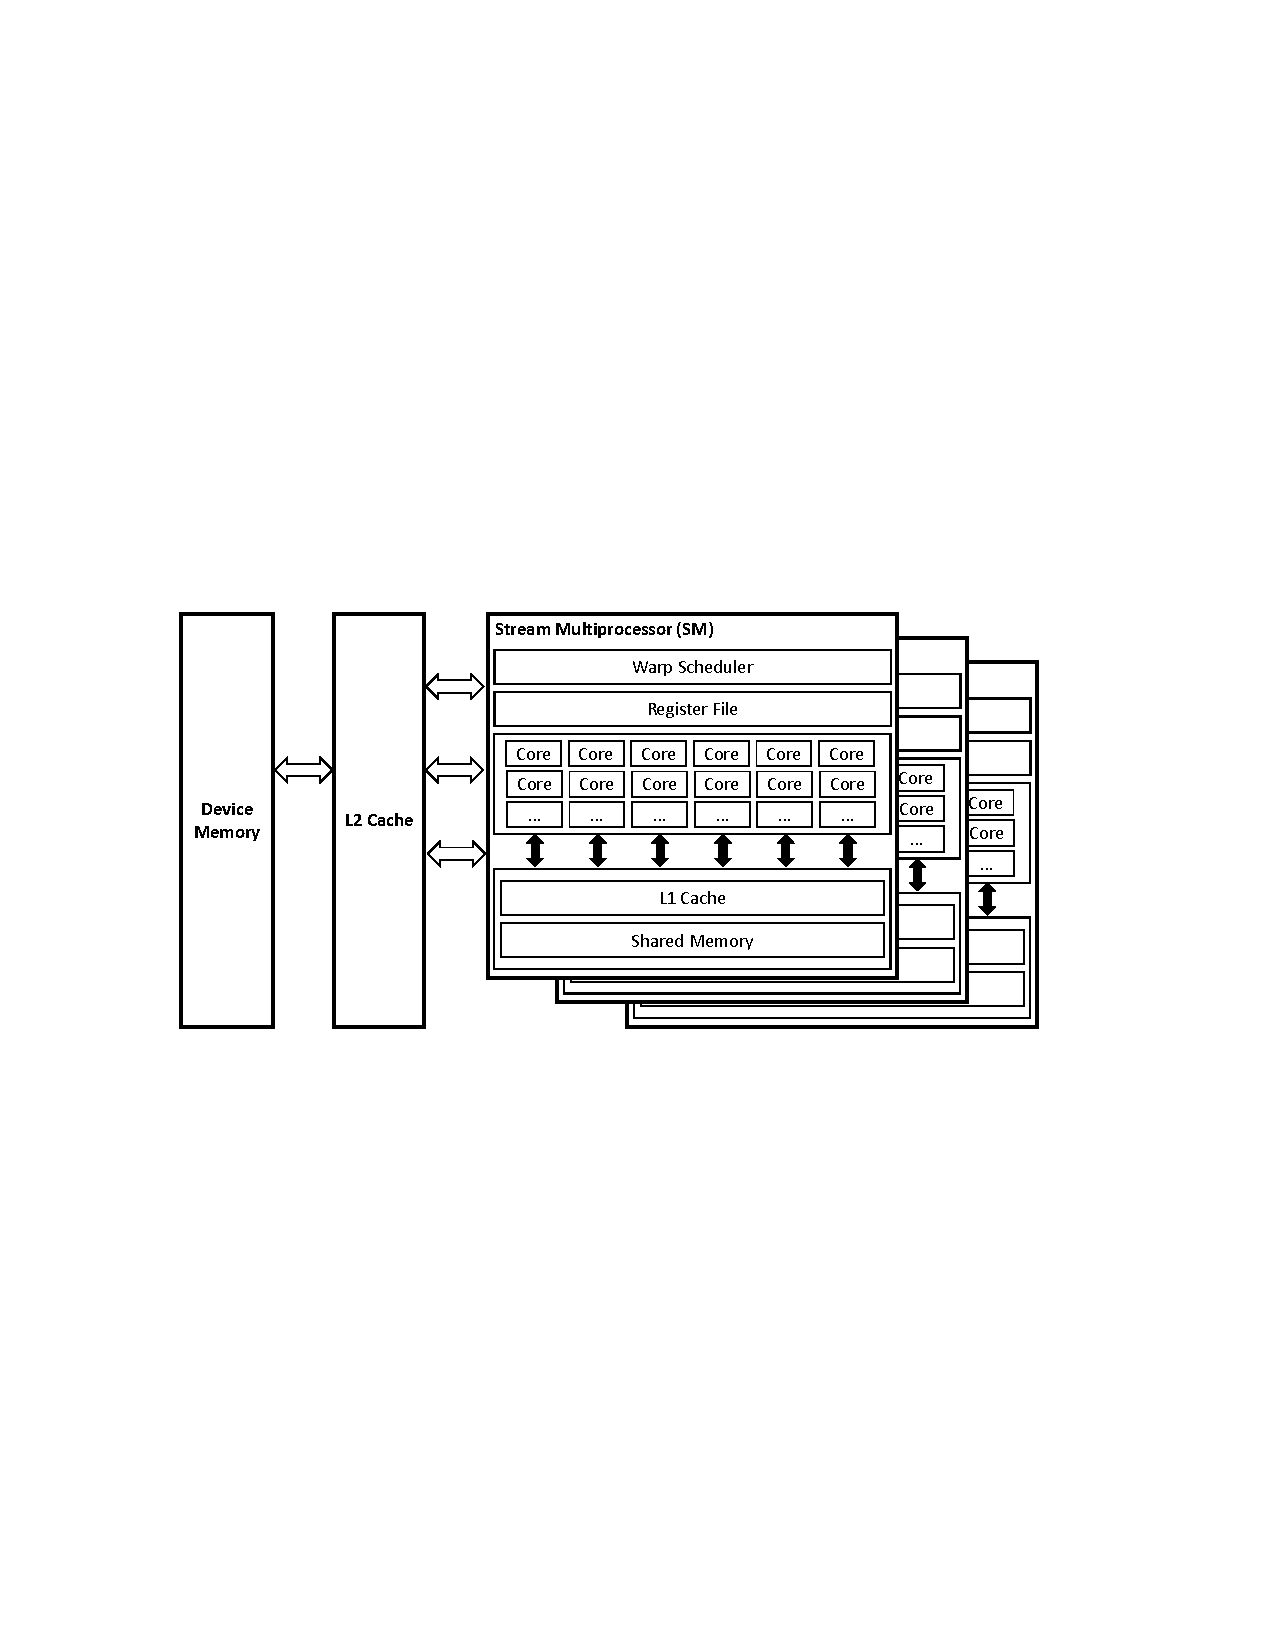
\includegraphics[width=0.5\textwidth]{fig/GPU-arch.pdf}
	\caption{Layout of an NVIDIA GPU architecture}
	\label{fig:arch}
\end{figure}

We introduce the background of the NVIDIA GPU architecture in this paper because its popularity and the wide adoption of the CUDA programming language. 
However, our proposed approaches are not unique to NVIDIA GPUs and can also be implemented on other GPU architectures. 
Figure~\ref{fig:arch} presents a high-level layout of a NVIDIA GPU. 
An application written in CUDA executes on GPUs by invoking the \emph{kernel} function. The kernel is organized as several \emph{thread blocks}, and one block executes all its threads on a \emph{streaming multiprocessor} (SM), which contains several CUDA cores as depicted in Figure~\ref{fig:arch}. Within each block, threads are divided into \emph{warps} of 32 threads each. 
A CUDA core executes the same instruction of a warp in lockstep.
Each warp runs independently, but warps can collaborate through different memory types as discussed in the following.  

\vspace{1mm}\noindent\textbf{Memory Hierarchy.} Compared to CPUs, GPUs are built with large register files that enable massive parallelism. 
%For example, NVIDIA GTX 1080 GPUs feature 256KB of register files for each SM. 
Furthermore, the shared memory, which has similar performance to L1 cache, can be programmed within a block to facilitate efficient memory access inside an SM.
The L2 cache is shared among all SMs to accelerate memory access to the device memory, which has the largest capacity and the lowest bandwidth in the memory hierarchy.

%GPUs offer an significant better data accessing throughputs than CPUs for two major reasons. 
%First,the device memory has high memory bandwidth, often an order of magnitude faster than RAM.
%Second, GPUs effectively hide memory access latency by warp switching. When a warp is blocked by memory accesses, other warps whose next instruction has its operands ready are eligible to be scheduled for execution. With sufficient threads launched, memory stalls can be minimized or even eliminated \cite{zhang2015mega}.
%Thus, the fast data accessing performance makes GPUs an ideal accelerator for data intensive applications such as hash tables. 

%Data is transferred between CPUs and GPUs (or between two GPU devices) via the PCIe link (Gen 3), which has been the bottleneck of many data-intensive applications \cite{zhang2015mega,kaldewey2012gpu,zhang2013omnidb}. In recent years, there have been many innovations proposed to reduce the overhead of the data transfer, from overlapping PCIe transfer with kernel execution to using hardware acceleration such as PCIe Gen 4 and NVlink \cite{thompto2016power9}. Nonetheless, we omit the discussion on how to minimize this data transfer cost since it is orthogonal to designing an efficient hash table on \emph{one} GPU device.

\vspace{1mm}\noindent\textbf{Optimizing GPU Programs.}
There are several important guidelines to harness the massive parallelism of GPUs.
\begin{itemize}
	\item \emph{Minimize Warp Divergence.} Threads in a warp will be serialized if executing different instructions. To enable maximum parallelism, one just minimize branching statements executed within a warp.  
	\item \emph{Coalesced Memory Access.} Warps have a wide cache line size. The threads are better off reading consecutive memory locations to fully utilize the device memory bandwidth, otherwise a single read instruction by a warp will trigger multiple random accesses. 
	\item \emph{Control Resource Usage.} Registers and shared memory are valuable resources for enabling fast memory accesses. Nevertheless, each SM has limited resources and overdosing register files or shared memory leads to reduced parallelism on a SM.  
	\item \emph{Atomic Operations.} When facing thread conflicts, an improper locking implementation causes serious performance degradation. One can leverage the native support of atomic operations \cite{sanders2010cuda} on GPUs to carefully resolve the conflicts and minimize thread spinning.
\end{itemize}
\section{related works}\label{sec:rel}
Alcantara \textit{et al.} present a seminar work on GPU-based cuckoo hashing to accelerate computer graphics workloads \cite{alcantara2009real}. 
This work has inspired a number of applications from diverse fields. Wu \textit{et al.} investigate the use of GPU-based cuckoo hashing for
on-the-fly model checking \cite{wu2015gpu}. A proposal of accelerating the nearest neighbor search is presented in \cite{pan2010efficient}. 
Due to the success of cuckoo hashing on GPUs, the implementation of \cite{alcantara2009real} has been adopted in the CUDPP library\footnote{https://github.com/cudpp/cudpp}.
To improve from \cite{alcantara2009real}, stadium hash is proposed in \cite{khorasani2015stadium} to support out-of-core GPU parallel hashing. However it uses double hashing which needs to rebuild the entire table for any deletions.  
Zhang \textit{et al.} propose another efficient design of GPU-based cuckoo hashing, named MegaKV, 
to boost the performance for KV store \cite{zhang2015mega}. 
Subsequently, Horton table \cite{breslow2016horton} improves the efficiency of \formal{find} over MegaKV by trading with the cost of introducing a KV remapping mechanism.
Meanwhile, in the database domain, several SIMD hash table implementations have been proposed to facilitate relation join and graph processing, including cuckoo hash \cite{ross2007efficient} and linear probing \cite{zhong2014medusa}. 

It is noted that the aforementioned works focus on the static case: the size of data that needs to be hashed is known in advance. Thus, the static designs would prepare a sufficiently large memory to store the hash table. In this way, the hash table operations are fast since the collision rarely happens. However, the static approach wastes memory resources and, to some extent, it prohibits other data structures for the same application to coexist on the device memory. 
%Moreover, existing designs rely on atomicExch
%operation to avoid conflicts when transacting a KV pair on GPUs, which only supports up to 64 bits for KV altogether. This design, albeit being efficient, has severe limitation as the value component exceeds 64 bits in many real-world scenarios.  
This motivates us to develop a general dynamic hash table on GPUs that actively makes adjustments according to the data size to preserve space efficiency. 
%In this paper, we propose a dynamic cuckoo hash table on GPUs, which maintains high filled factor to minimize memory footprint. In order to support efficient concurrent hash updates, we introduce a novel voter-based coordination scheme which reduces thread conflicts. 
%Experimental results have revealed that the proposed solution could achieve competitive or even better performance than the state-of-the-art static hash tables on GPUs, while utilizing significantly less device memory. 

To the best of our knowledge, there is only one existing work for building dynamic hash tables on GPUs \cite{ashkiani2018dynamic}.
This proposed approach presents a concurrent linked list structure, called \emph{slab list}, to construct the dynamic hash table with \emph{chaining}. 
However, there are three major issues for slab list. 
First, it could frequently invoke concurrent memory allocation requests, especially when the data keeps inserting. Efficient concurrent memory allocation is difficult to implement under the GPU architecture due to its massive parallelism. Although a dedicated memory management strategy is proposed in \cite{ashkiani2018dynamic} to alleviate this allocation cost, it is not transparent to other data structures. More specifically, the dedicated allocator still needs to reserve a large piece of memory in advance to prepare for efficient dynamic allocation, and the occupied space cannot be readily accessed by other GPU resident data structures. 
Second, slab list does not guarantee a fixed filled ratio against deletions. 
It symbolically marks a deleted entry without physically free the memory space. 
Hence, memory spaces are wasted when they were occupied by deleted entries. 
Third, the chaining approach has a lookup time of $\Omega(log(log(m)))$ for some KVs with high probability. This not only results in degraded performance for \formal{find}, but also triggers more overheads in resolving conflicts when multiple \formal{insert} and \formal{delete} operations occur at the same key.
In contrast, the cuckoo hashing table adopted in this work guarantees $\Theta(1)$ worst case complexity for \formal{find} and \formal{delete}, 
$O(1)$ amortized \formal{insert} performance. Moreover, we do not introduce extra complication in implementing customized memory manager but only reply on the default memory allocator provided by CUDA, and, at the same time, ensures fixed filled ratio for the hash tablec.
\section{Dynamic Hash Table}\label{sec:dyn}
In this section, we propose the resizing strategy against dynamic hash table updates on GPUs. We first present the hash table design in Section~\ref{sec:dyn:has}.
Subsequently, the resizing strategy is introduced in Section~\ref{sec:dyn:resize}.
In section~\ref{sec:dyn:distribute}, we discuss how to distribute the KV pairs for better load balancing with theoretical guarantees. 
Finally, we present how to efficiently rehash and relocate the data after the tables have been resized in Section~\ref{sec:dyn:rehash}. 

\subsection{Hash Table Structure}\label{sec:dyn:has}
Following cuckoo hashing \cite{pagh2004cuckoo}, we build $d$ hash tables with $d$ unique hash functions: $h^1,h^2,\ldots,h^d$. 
In this work, we use a set of simple universal hash functions such as $h^i(k) = (a_i\cdot k + b_i \mod p) \mod |h^i|$.
$a_i,b_i$ are random integers, $p$ is a large prime.
Note that the proposed approaches in this paper also apply to other hash functions as well. 
There are three major advantages for adopting cuckoo hashing on GPUs. 
First, it avoids chaining by inserting the elements into alternative locations if collision happens. As discussed in Section~\ref{sec:rel}, 
chaining presents several issues which are not friendly to the GPU architecture.  
Second, to lookup a KV pair, one only needs to search $d$ locations specified by $d$ unique hash functions. 
Thus, the data could be stored contiguously in the same location and enable the preferred coalesced memory access. 
Third, cuckoo hashing can maintain high filled factor, which is ideal for memory saving in the dynamic scenario. 
For $d=3$, cuckoo hashing achieves over $90\%$ filled factor and still processes \formal{insert} operations efficiently \cite{fotakis2005space}.

\begin{figure}[t]
	\centering
	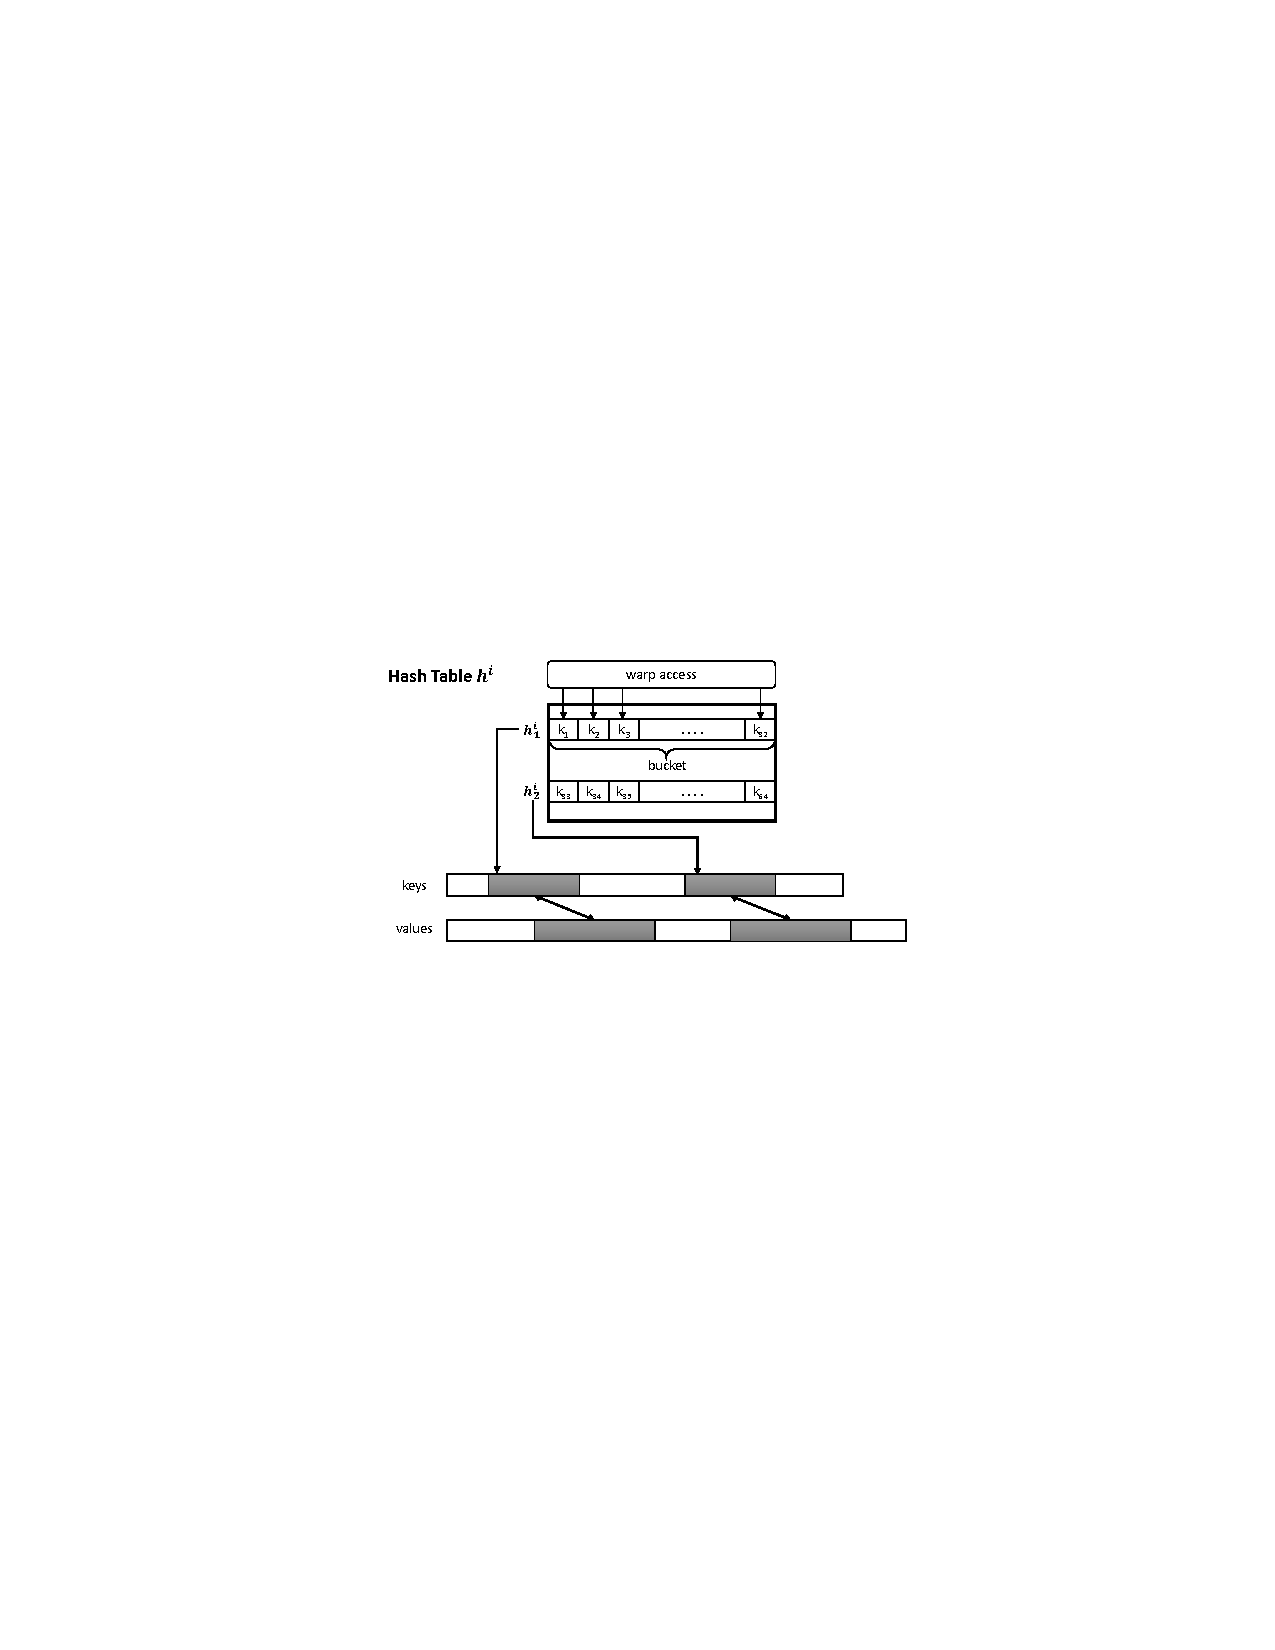
\includegraphics[width=0.45\textwidth]{fig/Hashtable.pdf}
	\caption{The hash table structure}
	\label{fig:hashtable}
\end{figure}

Figure~\ref{fig:hashtable} depicts the design of a single hash table $h^i$ on GPUs. 
Assuming the keys are 4-byte integers. A bucket of 32 keys, which are all hashed to the same value $h^i_j$, are stored consecutively in the memory. 
The design of buckets maximizes the utilization of memory bandwidth in GPUs. 
Consider the L1 cache line size is 128 bytes, only a single access is required when one warp is assigned to access a bucket. 
The values associated with the keys in the same bucket are also stored consecutively but in a separate array.   
In other words, we use two arrays to store the keys and the values respectively.
The values could take much larger memory space than the keys. 
Thus, storing keys and values separately avoids the overhead of memory access when accessing the values is not necessary, 
e.g., finding a nonexistent KV pair or deleting a KV pair. 

For keys having size larger than 4 bytes, a simple strategy is to store less KV pairs in a bucket. Suppose the keys are 8-bytes, a bucket can then accommodate 16 KV pairs. 
Furthermore, we lock the entire bucket exclusively for a warp to perform insertion/deletion using intra warp synchronization primitives. Thus, we do not limit ourselves to supporting KV pairs with only 64 bits. 
In the worst case, a key taking 128 bytes occupy one bucket alone, which is unnecessarily large in practice.

\subsection{Structure Resizing}\label{sec:dyn:resize}
To efficiently utilize GPU device memory, we resize the hash tables when the filled factor falls out of the desired range, e.g., $[\alpha,\beta]$.
One possible strategy is to double or half all hash tables and to then rehash all KV pairs. However, this simple strategy renders poor memory utilization and 
excessive overheads for rehashing. First, doubling the size of the hash tables results in filled factor immediately cut to half, while downsizing the hash tables to half the size followed by rehashing could only be efficient when the filled factor is significantly low (e.g., $40\%$), both of which scenarios are not resource friendly. Second, rehashing all KV pairs is expensive and it hurts the performance stability for most of the streaming applications since the entire hash table is subject to locking. 

We propose an alternative strategy, illustrated in Figure~\ref{fig:example-resize}. 
Given $d$ hash tables depicted in Figure~\ref{fig:example-resize},
we always double the smallest subtable or chop the largest subtable into half for upsizing or downsizing respectively, when filled factor falls out of $[\alpha,\beta]$. 
In other words, no subtable will be more than double the size as others. The strategy implies that we do not need to lock all hash tables and only to resize one, thus achieving better performance stability compared with the aforementioned simple strategy. 

\vspace{1mm}
\noindent\textbf{Filled factor analysis:}
Assuming there are $d'$ hash tables with size $2n$, $d-d'$ tables with size $n$ and the current filled factor $\theta$, 
one upsizing process when $\theta > \beta$ lowers the filled factor to $\frac{\theta\cdot(d+d')}{d+d'+1} \geq \frac{\beta \cdot d}{d+1}$.  
Since the filled factor is always lower bounded by $\alpha$, we can deduce that $\alpha < \frac{d}{d+1}$.
Apparently, a higher lower bound can be achieved by adding more hash tables, while it leads to less efficient \formal{find} and \formal{delete}. 
We allow the user to configure the number of hash tables to trade off memory and query processing efficiency. 

\begin{figure}[t]
	\centering
	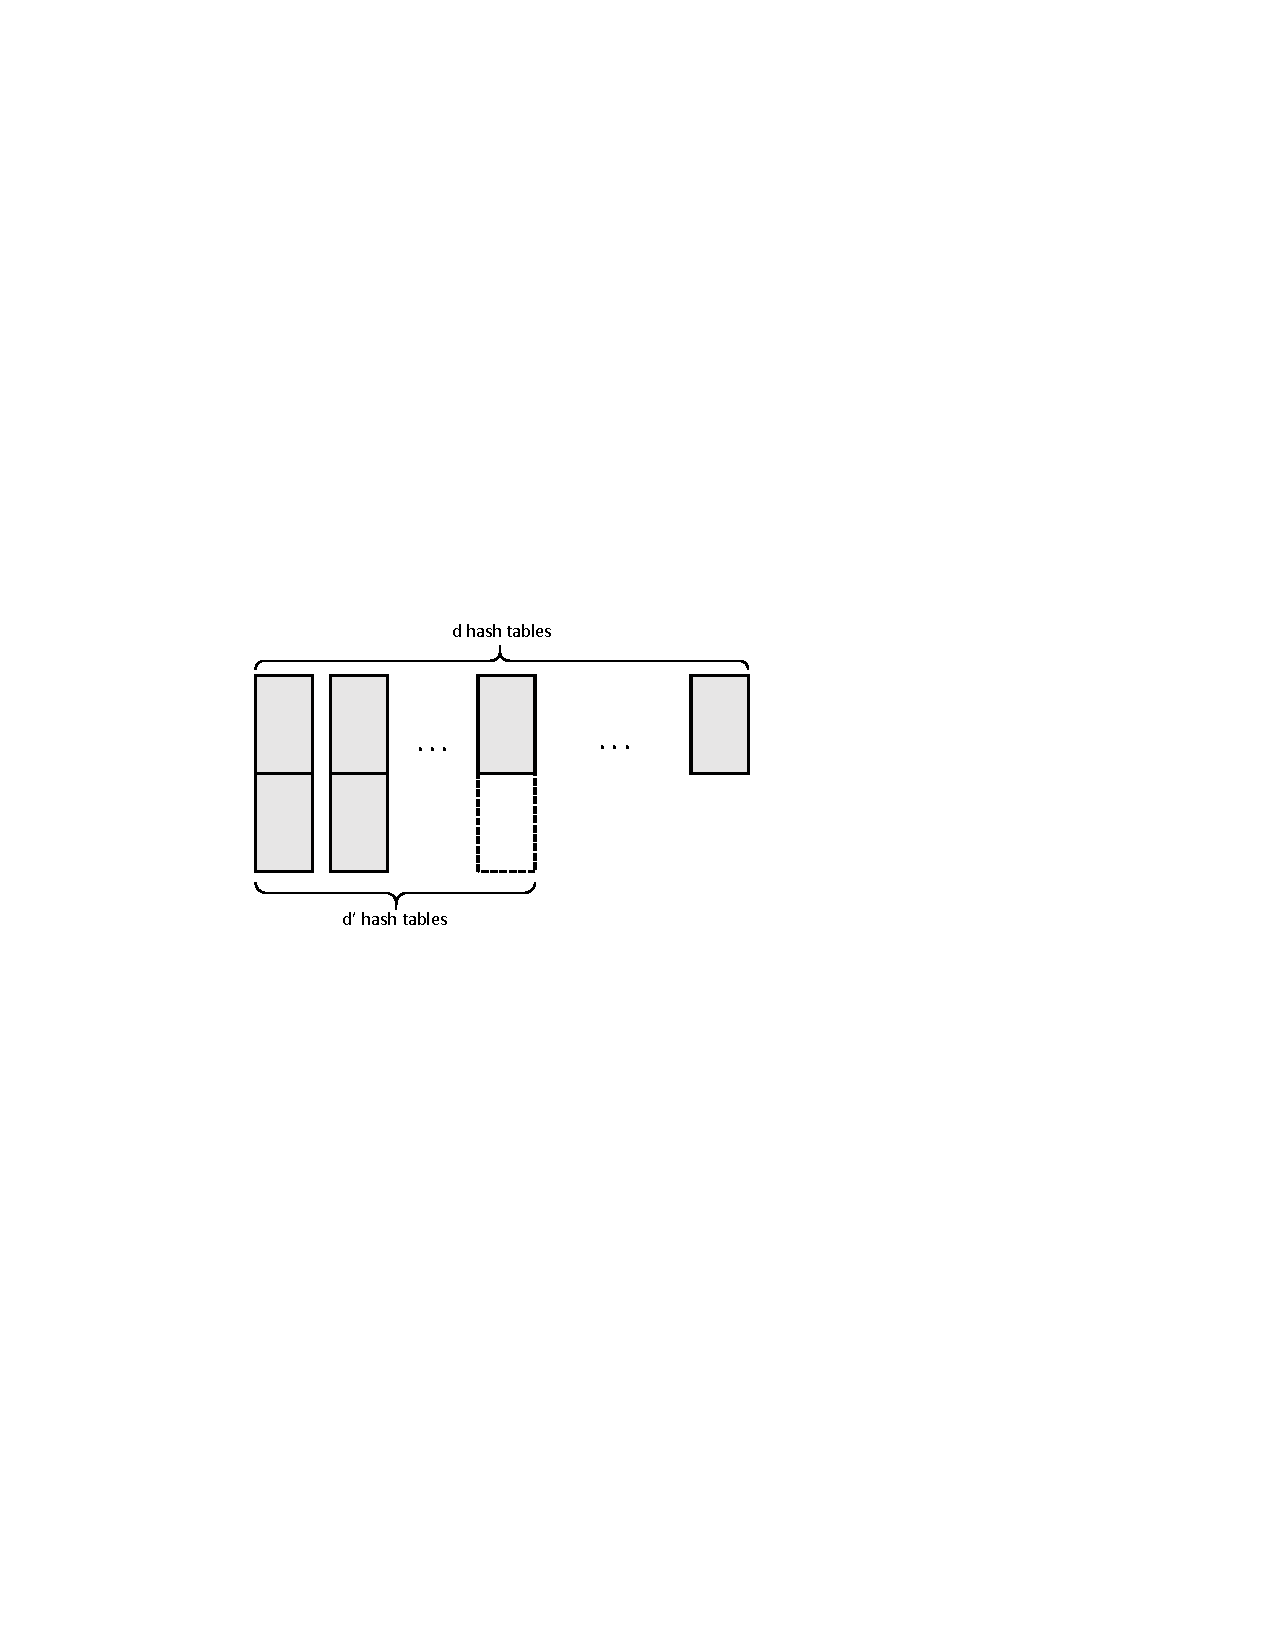
\includegraphics[width=0.35\textwidth]{fig/MultiTable.pdf}
	\caption{Resizing strategy}
	\label{fig:example-resize}
\end{figure}
\subsection{KV distribution}\label{sec:dyn:distribute}
Given a set of KV pairs to insert in parallel, it is critical to distribute the KV pairs among the hash tables in a way such that the hash collisions are minimized for reducing the corresponding thread conflicts. We have the following theorem to guide us for distributing the KV pairs. 

\begin{theorem}\label{them:balance}
	The amortized conflicts for inserting $m$ unique KV pairs to $d$ hash tables is minimized when $\binom{m_1}{2}/n_1 = \ldots = \binom{m_d}{2}/n_d$. 
	$m_i$ and $n_i$ denote the elements inserted to table $i$ and the size of table $i$, respectively.  
\end{theorem}
\begin{proof}
	It is noted that the amortized insertion complexity of cuckoo hash is $O(1)$. Thus, similar to balls and bins analysis, the expected number of conflicts occurred for inserting $m_i$ elements in table $i$ is estimated as $\binom{m_i}{2}/n_i$. Minimizing the amortized conflicts among all hash tables can be modeled as the following optimization problem:
	\begin{equation}\label{eq:conflict-min}
	\begin{array}{ll@{}ll}
	\min_{m_1,\ldots,m_d \geq 0} & \sum_{i=1,\ldots,d} \binom{m_i}{2}/n_i \\
	\text{s.t.} & \sum_{i=1,\ldots,d} m_i = m
	\end{array}
	\end{equation}
	To solve the optimization problem, we establish an equivalent objective function:
	\begin{align*}
	\min \sum_{i=1,\ldots,d} \frac{\binom{m_i}{2}}{n_i} \Leftrightarrow \min \log(\frac{1}{d}\sum_{i=1,\ldots,d} \frac{\binom{m_i}{2}}{n_i})
	\end{align*}
	By Jensen's inequality, the following inequality holds:
	\begin{align*}
	\log(\frac{1}{d}\sum_{i=1,\ldots,d} \frac{\binom{m_i}{2}}{n_i}) \geq \frac{1}{d}\sum_{i=1,\ldots,d}\log(\frac{\binom{m_i}{2}}{n_i})
	\end{align*}
	where the equality holds when $\binom{m_i}{2}/n_i = \binom{m_j}{2}/n_j$ $\forall i,j = 1,\ldots,d$ and we obtain the minimum.
\end{proof}

According to our resizing strategy, one hash table can only be as twice large as the other tables. 
This implies the filled factors of two tables are equal if they have the same size, i.e., $\theta_i = \theta_j$ if $n_i = n_j$, 
while $\theta_i \simeq \sqrt{2}\cdot \theta_j$ if $n_i = 2n_j$. 
Thus, larger tables should have a higher filled factor. 
Guided by Theorem~\ref{them:balance},
we employ a randomized approach: 
a KV pair $(k,v)$ will be firstly assigned to table $i$ with a probability proportional to $n_i/\binom{m_i}{2}$ to ensure the distribution of KVs.

\subsection{Rehashing}\label{sec:dyn:rehash}
Whenever the filled factor falls out of the desired range, rehashing relocates the KV pairs after one of the hash table is resized. An efficient relocation process maximizes the utilization of GPU device memory bandwidth and minimizes thread conflicts. 
We discuss two scenarios for rehashing: \emph{upsizing} and \emph{downsizing}. Both scenarios are processed in one single kernel. 

\begin{figure}[t]
	\centering
	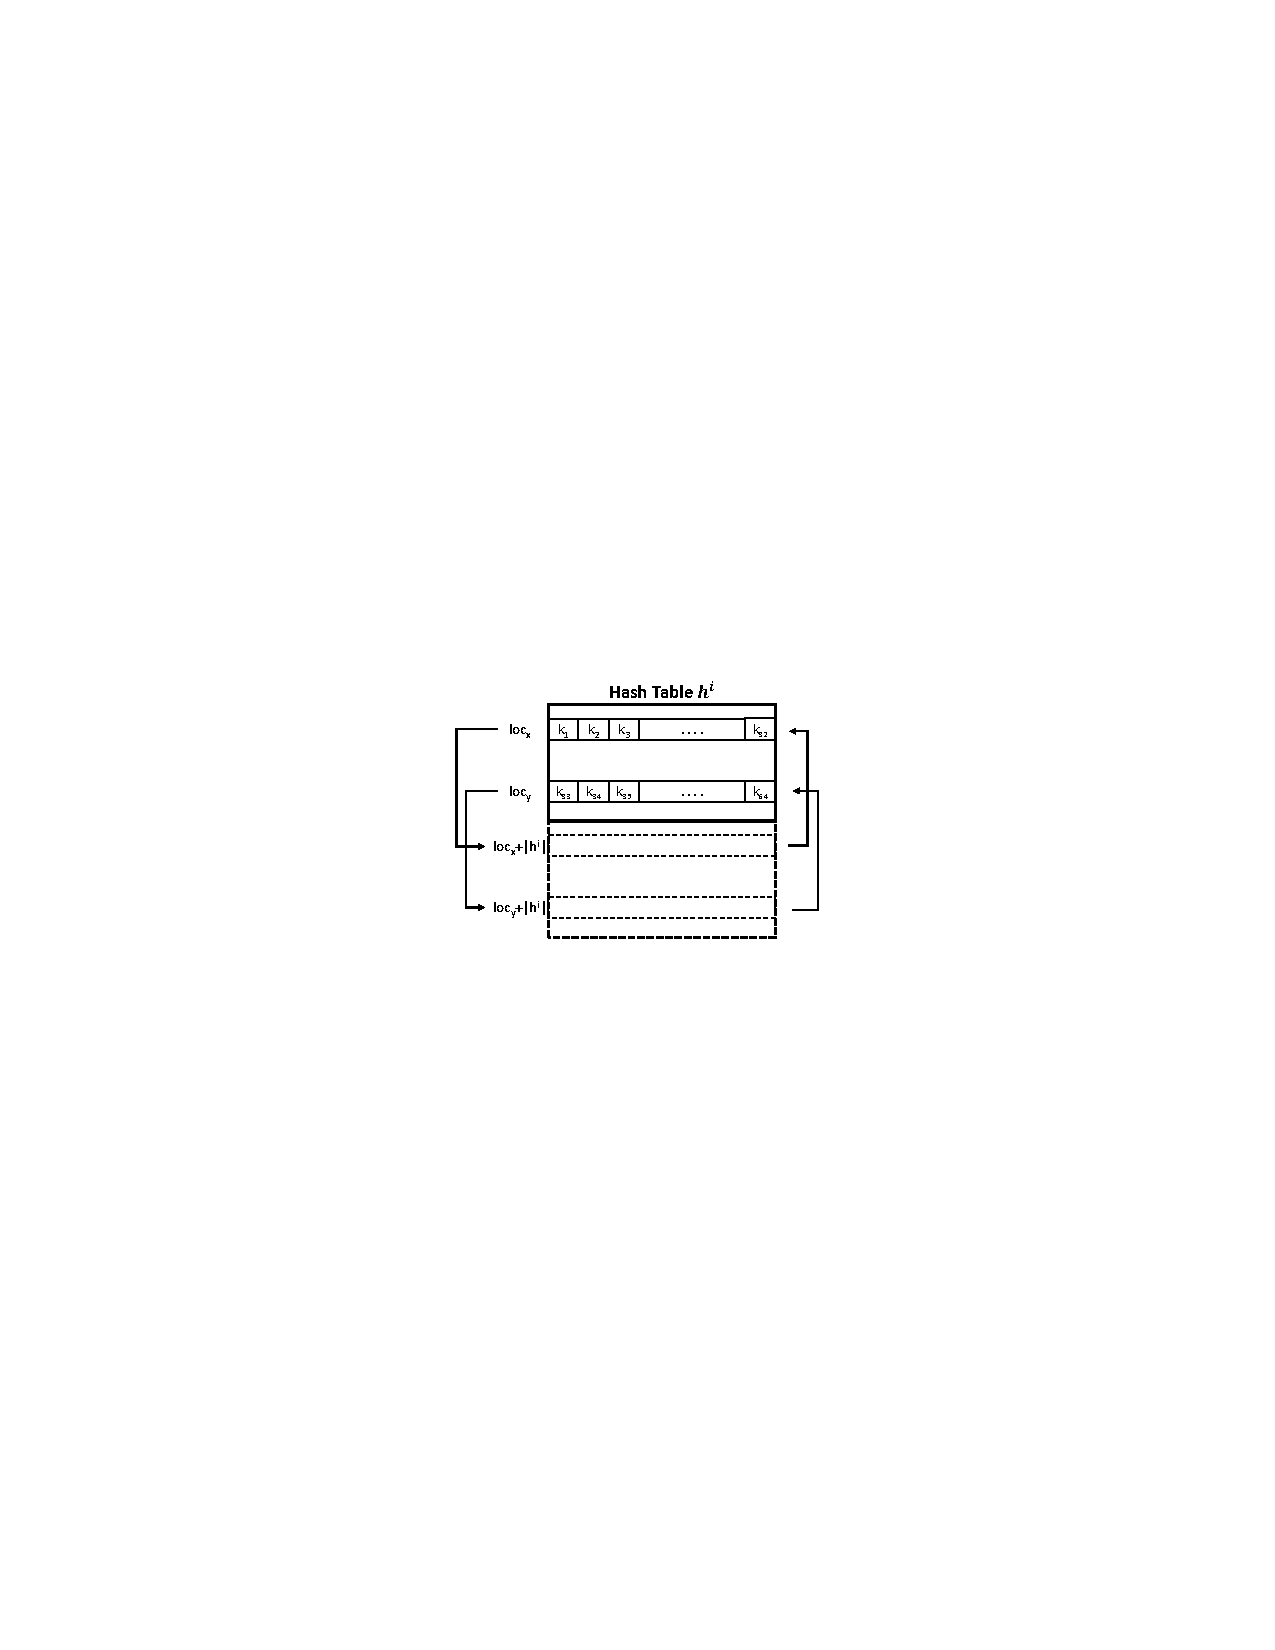
\includegraphics[width=0.3\textwidth]{fig/Upsize.pdf}
	\caption{Illustration for upsizing and downsizing.}
	\label{fig:upsize}
\end{figure}
\vspace{1mm}\noindent\textbf{Upsizing.} 
We introduce a conflict-free rehashing strategy for the upsizing scenario. 
Figure~\ref{fig:upsize} presents an illustration for upsizing a hash table $h^i$. 
As we always double the size for $h^i$, 
a KV pair which originally resides in bucket $loc$ could be rehashed to bucket $loc+|h^i|$ or stay in the original bucket. 
With this observation, we assign a warp for rehashing all KV pairs in bucket to fully utilize the cache line size. 
Each thread in the warp corporately takes a KV pair in the bucket and relocates the KV pair if necessary.
Moreover, the rehashing does not trigger any conflict since KV pairs from two distinct buckets before upsizing cannot be rehashed to the same bucket.  
Thus, the locking of a bucket is not required, and we can make use of the full device memory bandwidth for the upsizing process.  

Note that after upsizing hash table $h^i$, its filled factor $\theta_i$ is cut to half, which could break the balancing condition emphasized in Theorem~\ref{them:balance}. Nevertheless, we use the sampling strategy for subsequent KV insertions, where each insertion is allocated to table $i$ with a probability proportional to $n_i/\binom{m_i}{2}$, to recover the balancing condition. In particular, $m_i$ remains the same while $n_i$ doubles after upsizing, the scenario leads to double the probability of inserting subsequent KV pairs to $h^i$. 


\vspace{1mm}\noindent\textbf{Downsizing.}
Downsizing the hash table $h^i$ is a reverse process of upsizing $h^i$. We note that there is always room to relocate KV pairs in the same table for upsizing. 
In contrast, downsizing may rehash some KV pairs to other hash tables, especially when $\theta_i > 50\%$.
Since the KV pairs located in $loc$ and $loc+|h^i|$ are hashed to $loc$ in the new table, there could be cases the KV pairs exceeds the size of a single bucket. 
Hence, we first assign a warp to accommodate KV pairs that can fit the size of a single bucket. Similar as upsizing, it does require locking since there will be no thread conflict on any bucket. 
For the remaining KV pairs which cannot fit in the downsized table, called \emph{residuals}, we insert them into other subtables.
To make sure no conflict occurs between inserting residuals and processing the downsizing subtable, which are both executed in a single kernel, we exclude the downsizing subtable when inserting the residuals. 
Take an example when we have three subtables and one of them is being downsized. 
We only insert the residuals to the remaining two subtables. 


%To safeguard the balancing condition, we devise a different rehashing strategy for downsizing. 
%For all KV pairs in bucket $loc \geq |h^i|/2$ for table $i$ to be downsized, we assign a thread to rehash and reinsert a KV pair using Algorithm~\ref{algo:insert}. 
%In this way, we achieve the balancing condition at the expense of locking a bucket when reinserting a KV pair. 

\vspace{1mm}\noindent\textbf{Complexity Analysis.}
Given a total of $m$ elements in the hash tables, upsizing/downsizing rehashes at most $m/d$ KV pairs. 
For inserting/deleting these $m$ elements, the number of rehashes is bounded by $2m$. 
Thus, the amortized complexity for inserting $m$ elements is still $O(1)$.




\section{Two-layer Cuckoo Hash}\label{sec:vot}
In this section, we present the two-layer approach that ensures at most two lookups for \formal{find} and \formal{delete} (Section~\ref{sec:vot:two}). 
Subsequently, in Section~\ref{sec:vot:con}, we give details on optimizing GPUs for paralleling hash table operations, i.e., \formal{find}, \formal{insert} and \formal{delete}.


%\begin{algorithm}[t]
%	\begin{algorithmic}[1]
%		\State $found \gets \emptyset$
%		\For{$i=0,\ldots,d-1$}
%		\State $loc \gets h^i(k)$
%		\State $found \gets ballot(loc[l].key == k)$
%		\If{$found \neq \emptyset$}
%		\State \Return $loc[l]$
%		\EndIf
%		\EndFor
%		\State \Return false
%	\end{algorithmic}
%	\caption{\textbf{Find}(lane $l$, warp $wid$, key $k$)}\label{algo:find}
%\end{algorithm}

\subsection{The Two-layer Approach}\label{sec:vot:two}
Given the proposed dynamic hash table design, it is noted that a larger $d$ implies smaller workload for each resizing operation, as each single table will be smaller with fixed filled factor. On top of efficient resizing, higher filled factor can be maintained as discussed in Section~\ref{sec:dyn:resize} for larger $d$. Nevertheless, the benefit of employing more tables does not come for free. For each \formal{find} and \formal{delete} operations, one has to perform $d$ lookups, which translate to $d$ random accesses to the device memory. 
Random accesses are particularly expensive as GPUs contain limited cache size and simplified control units compared with those of CPUs.

One possible approach to reduce the number of lookups is to first hash all KV pairs into $d'$ partitions. For each partition, we employ a cuckoo hash with two hash functions. In this way, one only needs to perform two lookups for any \formal{find} and \formal{delete} operations. However, this approach cannot prevent the skewness issue across the $d'$ partitions, especially against frequent delete operations. It is possible that the deleted KVs all fall into one partition $c_i$, which results in low filled factor for the table/s allocated to $c_i$. Furthermore, when inserting KVs into other partitions, e.g., $c_j \neq c_i$, the efficiency could be severely degraded due to high filled factor of the table/s allocated to $c_j$. 

Hence, we propose a two-layer approach to resolve the skewness issue.
\revise{
The two-layer approach is inspired by the data partitioning technique~\cite{bender2012don,boncz1999database,zhang2019data,zuo2018write}. 
}
Given $d$ hash tables, we first hash all KV pairs into $\binom{d}{2}$ partitions. 
Each partition refers to a unique pair of hash tables. Then, each KV pair is hashed and stored in only one of corresponding pair. In this way, it only requires at most two lookups for \formal{find} and \formal{delete}. The advantage of this approach is that each KV pair could appear in any of the $d$ hash tables, which offers opportunities to balance a skewed distribution. The following example illustrates a scenario where the skewness is mitigated during the insertion process. 

\begin{example}
A KV pair $(k,v)$ is hashed to the pair $(h_i,h_j)$ for the first layer,  we will then hash $k$ and try to insert $(k,v)$ into $h_i$ for the second layer. Assuming the corresponding bucket in $h_i$ is full for $(k,v)$, we evict another KV pair $(k',v')$. Then, we discover that $(k',v')$ is hashed to the pair $(h_i,h_t)$. Henceforth, we insert $(k',v')$ to $h_t$ and the process repeats until no eviction.
\end{example}

From the above example, we can see that the eviction could reinsert a KV pair into any hash table $h_t$. As each filled bucket contains 32 KV pairs (assuming the keys are 4 bytes), one can pick a KV pair for re-insertion into a desired hash table based on the balancing strategy discussed in Theorem~\ref{them:balance}. In addition to the ability for mitigating data skewness, we can show that two-layer cuckoo hash has the same asymptotically insertion performance as that of the plain cuckoo hash table with two hash functions.  

\begin{theorem}\label{them:complexity}
The two-layer cuckoo hash approach has the same expected, amortized complexity of insertion as that of the plain cuckoo hash with two hash tables. 
\end{theorem}

\begin{proof}
Assuming $d$ hash tables for the two-layer approach, W.L.O.G. we set $[0,n)$ to be the range for each hash function. Given a KV pair $(k,v)$, we denote that hash function $hp$ as the one which hashes $(k,v)$ to a pair of hash tables.
Now, we transform the two-layer approach to the plain cuckoo hash as the following:
we construct two new hash functions $H_1(k) = i \cdot n \cdot h_i(k)$ and $H_2(k) = j \cdot n \cdot h_j(k)$ where $hp(k) = (h_i,h_j)$.
Apparently, the range of $H_1$ and $H_2$ is $[0,nd)$. Thus, we can build a random bipartite graph $G(U,V,E)$ where the $U$ are the buckets for $H_1$, $V$ are the buckets for $H_2$ and $E$ are the KV pairs connecting two buckets from $H_1$ and $H_2$ respectively. 
We note that each KV pair is hashed to a random edge $e \in E$ with the same probability independently, i.e., $1/(n^2d^2)$. Hence, we can follow the similar proof procedure, which utilizes random bipartite graph analysis to show the amortized complexity for cuckoo hash with two tables \cite{kutzelnigg:hal-01184689}, to prove Theorem~\ref{them:complexity}.
\end{proof}



\subsection{Parallel Hash Table Operations}\label{sec:vot:con}
In the reminder of this session, we discuss how to utilize GPUs for the two-layer cuckoo hash. Following existing works \cite{alcantara2009real,zhang2015mega,breslow2016horton}, we assume the \formal{find}, \formal{insert} and \formal{delete} operations are batched and each batch only contains one type of operations. 
%A batch with mixed type of operations can also be supported but the semantic is ambiguous. 

\begin{figure}[t]
	\centering
	\hspace{-3em}
	\begin{minipage}{0.5\linewidth}
		\label{fig:atomicCAS}
		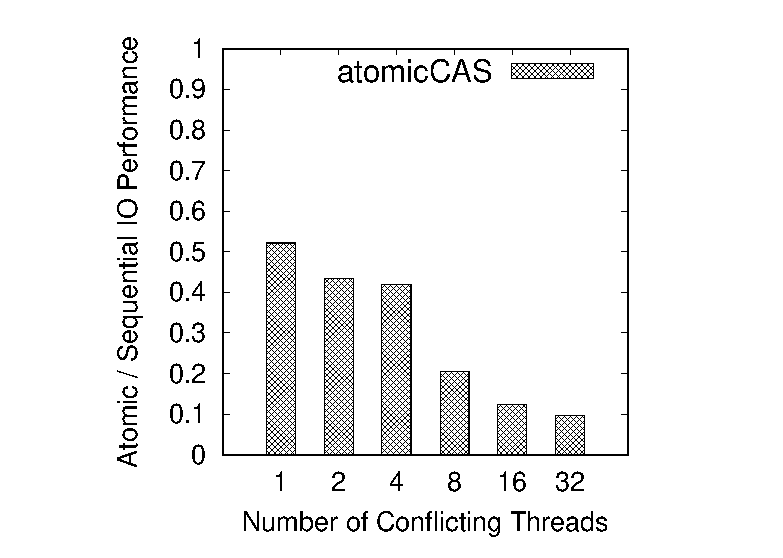
\includegraphics[width=5.3cm]{exp/atomic/atomicCAS.eps}
	\end{minipage}
	\hspace{-1em}
	\begin{minipage}{0.5\linewidth}
		\label{fig:atomicExch}
		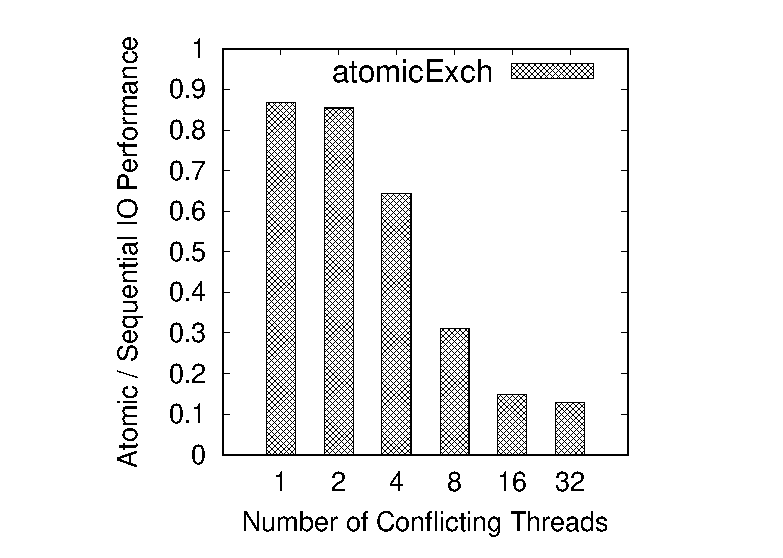
\includegraphics[width=5.3cm]{exp/atomic/atomicExch.eps}
	\end{minipage}
	\caption{The performance of atomic operations for increasing conflicts}
	\label{fig:atomic}
\end{figure}

\vspace{1mm}\noindent\textbf{Find.} It is relative straightforward to parallelize \formal{find} operations since only read access is required. 
Given a batch of size $m$, we launch $w$ warps in total (which means launching $32w$ threads in total) and each warp is responsible for $\floor{\frac{m}{w}}$ \formal{find} operations. To locate a KV, we need to hash the key to a hash table pair $(h_i,h_j)$ and perform at most two lookups in the corresponding buckets of $h_i$ and $h_j$ respectively. 
%Algorithm~\ref{algo:find} presents the pseudo code for a KV lookup by a warp. 
%First, the bucket of the $i$th hash table is located, i.e., $loc_i$.
%Then, each thread in the warp (a thread lane $l$) simultaneously searches the key and the ballot function return the lane for which the key is found.




\vspace{1mm}\noindent\textbf{Insert.} Contention occurs when multiple \formal{insert} operations target at the same bucket. 
There are two contrasting objectives for resolving the contention. On one hand, we want to utilize the warp-centric approach to access a bucket.
On the other hand, a warp requires a mutex when updating a bucket to avoid corruption, and the locking is expensive on GPUs.  
In the literature, it is a common practice to use atomic operations for implementing a mutex under the warp-centric approach \cite{zhang2015mega}. 
In particular, we can still invoke a warp to insert a KV pair. The warp is required to acquire a lock before updating the corresponding bucket. 
The warp will keep trying to acquire the lock before successfully obtain the control. 
There are two drawbacks for this direct warp-centric approach. 
First, the conflicting warps are spinning while locking, thus wasting computing resources.
Second, although atomic operations are supported by recent GPU architectures natively, 
they become costly when the number of atomic operations issuing at the same location increases. 
In Figure~\ref{fig:atomic}, we show the profiling statistics for two atomic operations which are often used to lock and unlock a mutex: atomicCAS and atomicExch respectively. 
We compare the throughputs of the atomic operations vs. an equivalent amount of sequential device memory IOs (coalesced) and present the trend for varying the number of conflicting atomic operations. It is apparent that the atomic performance has seriously degraded when a larger number of conflicts occur. 
Thus, it will be expensive for the direct warp-centric approach in the contention critical cases. 
Imaging one wants to track the number of retweets posted to active twitter accounts in the current month, via storing the twitter ID and the obtained retweet counts as KV pairs. In this particular scenario, certain twitter celebrities could receive thousands of retweets in a very short period. 
This triggers the same twitter ID gets updated frequently and a serious number of conflicts would happen. 




To alleviate the cost of spinning, we devise the voter coordination scheme. 
We assign an \formal{insert} to a thread rather than using a warp to handle the operation. Before submitting a locking request and updating the corresponding bucket, the thread will participate in a vote among the threads in the same warp. 
The winner thread $l$ becomes the leader of the warp and takes control. Subsequent, the warp inspects the bucket and insert the KV for $l$ if there are spaces left, upon $l$ successfully obtaining the lock.
If $l$ fails to get the lock, the warp revotes another leader to avoid locking on the same bucket.
Compared with locking on atomic operations, the cost of warp voting is almost negligible since it is heavily optimized in the GPU architecture.  


\begin{algorithm}[t]
	\begin{algorithmic}[1]
		\State $active \gets 1$	\label{algo:insert:active:start}
		\While{true}
		\State $l' \gets ballot(active == 1)$ \label{algo:insert:vote:start}
		\If{$l'$ is invalid}
		\State break \label{algo:insert:active:end}
		\EndIf
		\State $[(k',v'),i'] \gets broadcast(l')$ \label{algo:insert:lock:start}
		\State $loc = h^{i'}(k')$
		\If{$l' == l$}
		\State $success \gets lock(loc)$ \label{algo:insert:lock:end}
		\EndIf
		\If{$broadcast(success,l') ==$ failure}
		\State continue					\label{algo:insert:vote:end}
		\EndIf
		\State $l^* \gets ballot(loc[l].key == k' || loc[l].key ==\emptyset)$ \label{algo:insert:write:start}
		\If{$l^*$ is valid and $l' == l$}
		\State $loc[l^*].(key,val) \gets (k',v')$
		\State $unlock(loc)$
		\State $active \gets 0$;
		\State continue			\label{algo:insert:write:end}
		\EndIf
		\State $l^* \gets ballot(loc[l].key \neq \emptyset)$
		\If{$l^*$ is valid and $l' == l$}
		\State $swap(loc[l^*].(key,val),(k',v'))$
		\State $unlock(loc)$ \label{algo:insert:loop:end}
		\EndIf
		\EndWhile
	\end{algorithmic}
	\caption{\textbf{Insert}(lane $l$, warp $wid$)}\label{algo:insert}
\end{algorithm}

Parallel insertion with the voter coordination scheme is presented in Algorithm~\ref{algo:insert}.
The pseudo code demonstrates how a thread (with lane $l$) from warp $wid$ inserts a KV. 
\revise{The warp first conducts a vote with the ballot function among active threads and the process will terminate if all threads finish their tasks} (lines~\ref{algo:insert:active:start}-\ref{algo:insert:active:end}).  
This achieves better resource utilization since no thread will be idle when one of the threads in the same warp is active.  
The leader $l'$ then broadcasts its KV pair $(k',v')$ as well as the hash table $h_{i'}$ to the warp and tries to lock the inserting bucket (lines~\ref{algo:insert:lock:start}-\ref{algo:insert:lock:end}). 
\revise{Note that the ballot and broadcast functions are implemented with CUDA primitives $\_\_ballot$ and $\_\_shfl$.}
The broadcast function ensures all threads in the warp receive the locking result and the warp revotes if $l'$ fails to obtain the lock.
Otherwise, the warp follows $l'$ and proceeds to update the bucket for $(k',v')$ with a warp-centric approach similar to \formal{find}.
Once a thread finds $k'$ or an empty space in the bucket, $l'$ will add or update with $(k',v')$ (lines~\ref{algo:insert:write:start}-\ref{algo:insert:write:end}).
When there is no empty slot, $l'$ swaps $(k',v')$ with another KV $(k^*,v^*)$ in the bucket and inserts the evicted KV to hash table $j$ in the next round. 
The warp finishes the work when all KV pairs are inserted.
%In summary, each iteration of the loop presented in Algorithm~\ref{algo:insert} issues $1$ atomic operation and at most $1$ device memory read/write (lines~\ref{algo:insert:vote:start}-\ref{algo:insert:loop:end}).  

\vspace{1mm}
\revise{
\noindent\textbf{Implementation Details.} We use atomicCAS and atomicExch functions for locking and unlocking a bucket, respectively.
$atomicCAS(address,compare,val)$ reads the value $old$ located at the address $address$ in global or shared memory and computes $old == compare \;?\; val : old$, and stores the result back to memory at the same address.The function returns the value $old$. $atomicExch(address,val)$ reads the value $old$ located at the address $address$ in global or shared memory and stores $val$ back to memory at the same address. 
To implement the lock, we initialize a lock variable $lock$ for each bucket to be $0$. 
We lock the bucket using $atomicCAS(\&lock,0,1)$ and the lock is successful if the function returns $0$. 
We unlock the bucket by using $atomicExch(\&lock,0)$. 
}

%Note that we have yet covered how to choose the hash table index $i$ for each insertion (Algorithm~\ref{algo:insert}). Additional number of conflicts would happen if all threads attempting to insert to the same table. For the flow of presentation, we leave the discussion to Section~\ref{sec:dyn} since choosing the hash table is more coherent to the load balancing problem for resizing hash tables. 
%Moreover, a careful reader would find that the insertion process could lead to multiple appearances of the same key in different hash tables. To fill this gap, one can attach a timestamp to the insertion batch.
%Hence, the \formal{find} operation is required to scan all $d$ buckets of the same key and extracts the one with the latest timestamp.




We give the following example to demonstrate the parallel insertion process.
\begin{example}
	In Figure~\ref{fig:voter}, we visualize the scenario for three threads: $l_x$, $l_y$, $l_z$ from warp $a$ and warp $b$, inserting KV pairs $(k_1,v_1)$, $(k_{33},v_{33})$, $(k_{65},v_{65})$ independently. 
	Suppose $l_y$ and $l_z$ become the leaders of warp $a$ and $b$ respectively. Both threads will compete for the bucket $y$ and $l_z$ wins the battle. 
	$l_z$ will then leads warp $b$ to inspect the bucket and evict $(k_{64},v_{64})$ by replacing with $(k_{65},v_{65})$. 
	In the meanwhile, $l_y$ does not lock on bucket $y$ and joins the new leader $l_x$ voted in warp $a$. 
	$l_x$ locks bucket $x$ and inserts $(k_1,v_1)$ in place. Subsequently, $l_y$ may get back the control of warp $a$ and update $k_{33}$ with $(k_{33},v_{33})$ at bucket $y$. In parallel, $l_z$ locks bucket $z$ and inserts the evicted KV $(k_{64},v_{64})$ into the empty space. 
\end{example}

\vspace{1mm}\noindent\textbf{Delete.} The \formal{delete} operation, in contrast to \formal{insert}, does not require locking with a warp-centric approach. 
Similar to \formal{find}, we assign a warp to process a key $k$ on deletion. The warp iterates through the buckets among all $d$ hash tables that could possibly contain $k$. Each thread lane in the warp is responsible for inspecting one position in a bucket independently, and only erase the key if $k$ is found, thus causes no conflict.

%\begin{algorithm}[t]
%	\begin{algorithmic}[1]
%		\For{$i=1,\ldots,d$}
%			\State $loc \gets h^i(k)$
%			\State $found \gets (loc[l].key == k)$
%			\If{$found$}
%				\State $loc[l].key \gets \emptyset$
%			\EndIf
%		\EndFor
%	\end{algorithmic}
%	\caption{\textbf{Delete}(lane $l$, warp $wid$, key $k$)}\label{algo:delete}
%\end{algorithm}


\begin{figure}[t]
	\centering
	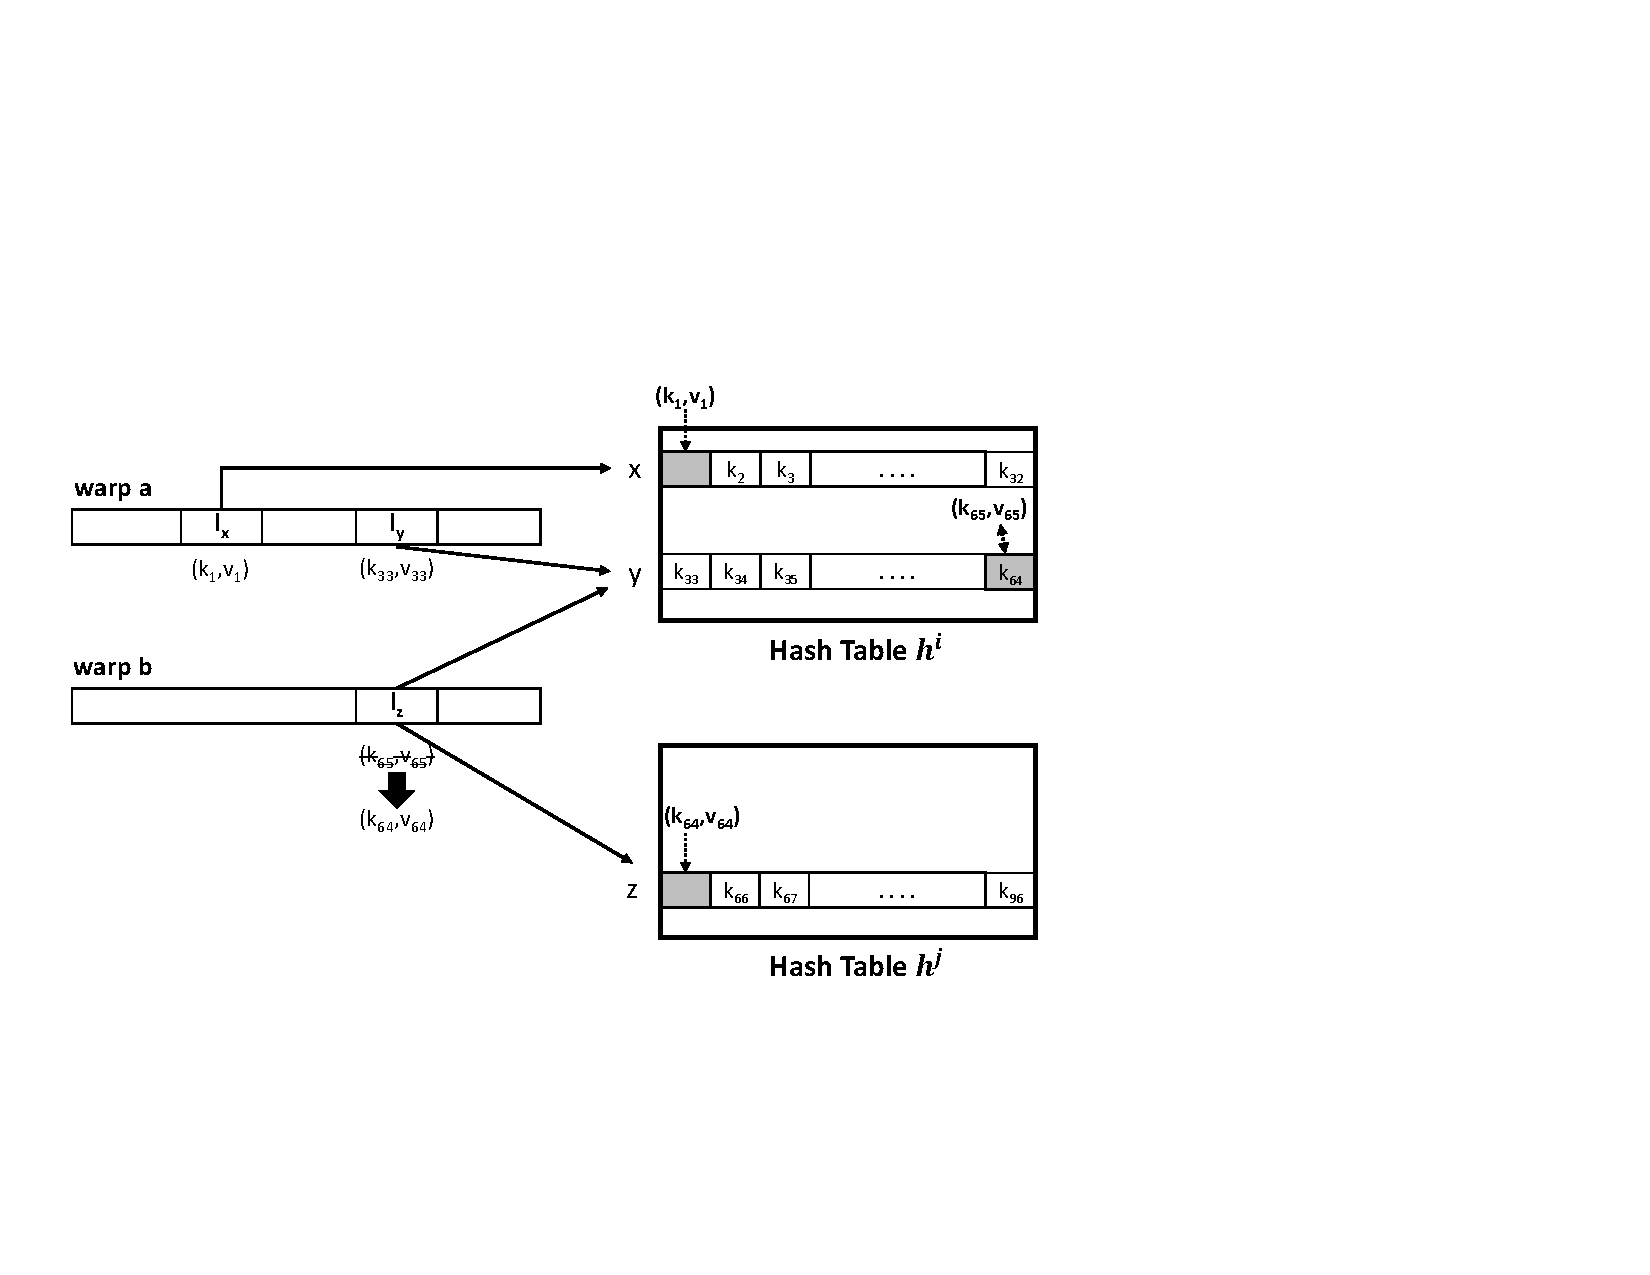
\includegraphics[width=0.48\textwidth]{fig/Voter.pdf}
	\vspace{-1em}
	\caption{Example for parallel insertions}
	\label{fig:voter}
\end{figure}
\vspace{1mm}\noindent\textbf{Complexity.}
Since a \formal{find}, \formal{insert} and \formal{delete} operation is independently executed by a thread. 
The analysis of a single thread complexity is the same as the sequential version of cuckoo hashing \cite{pagh2004cuckoo}: $O(1)$ worst case complexity for \formal{find} and \formal{delete}, $O(1)$ expected time for \formal{insert} for the case of 2 hash tables. 
It has been pointed out that analyzing the theoretical upper bound complexity of insertion in $d \geq 3$ hash tables is hard \cite{alcantara2009real}.  
Nevertheless, empirical results have shown that increasing the number of tables leads to better insertion performance. Please refer to our experimental results presented in Section~\ref{sec:exp}.
%Thus, we assume the complexity for inserting to $d$ hash tables is the same as that of $2$ has tables, as long as $d$ keeps constant.  

We then analyze the number of possible thread conflicts. Assuming we launch $m$ threads in parallel, each of them is assigned to a unique key, and the total number of unique buckets are $H=\sum_{i=1}^d|h^i|$. For \formal{find} and \formal{delete}, there is no conflict at all. 
For \formal{insert}, computing the expected number of conflicting buckets resembles the \emph{balls and bins} problem \cite{raab1998balls}, which is $O(\binom{m}{2}/H)$. 
Given GPUs have a large number of threads, there could be a significant amount of conflicts. Thus, we propose the voter coordination scheme to reduce the cost of spinning on locks. 
%Note that the analysis is done for the cases where the key to update is unique. More conflicts could occur in reality when the same key is updated in parallel. 
\section{experimental evaluation}\label{sec:exp}
In this section, we conduct extensive experiments by comparing the proposed hash table design \voter with several state-of-the-art approaches for GPU-based hash tables. 
Section~\ref{sec:exp:setup} introduces the experimental setup. 
Section~\ref{sec:exp:tune} presents the discussion on the sensitivity analysis of \voter.
In Sections~\ref{sec:exp:static} and \ref{sec:exp:dynamic}, we compare all approaches under the static and the dynamic experiments respectively.

\subsection{Experiment Setup}\label{sec:exp:setup}

\vspace{1mm}\noindent\textbf{Baselines.} We compare \voter with several state-of-the-art hash table implementations on GPUs. which are listed as the following:
\begin{itemize}
	\item \cudpp is a popular CUDA primitive library\footnote{https://github.com/cudpp/cudpp} which contains the cuckoo hash table implementation published in~\cite{alcantara2009real}. 
	For \cudpp, each hash value stores only one KV pair with 64 bits size (32 bits for key and 32 bits for value). 
	\cudpp only supports \formal{insert} and \formal{find} operations. We use the default setup of \cudpp which automatically chooses the number of hash functions based on the data to be inserted.
	\item \megakv is a warp-centric approach for GPU-based key value store published in~\cite{zhang2015mega}. \megakv employs a cuckoo hash with two hash functions and
	it allocates a bucket for each hash value. However, it does not lock a bucket when performing update. Instead, it uses intra-block synchronization to resolve race condition. 
	\item \slab is a state-of-the-art GPU-based dynamic hash table \cite{ashkiani2018dynamic}, which employs chaining and dedicated memory allocator for resizing.
	%\item \google is an efficient CPU-based hash table implementation\footnote{https://github.com/sparsehash/sparsehash-c11/}. We choose the \emph{dense\_hash\_map} implementation since it provides the best efficiency.
	\item \voter is the approach proposed in this paper.
\end{itemize}
We adopt the original implementations of the compared baselines from their corresponding inventors. 
%For \megakv, we note that its intra-block synchronization could lead to inconsistency issue as well as a large number of insertion failures, especially when the filled factor is high.  
%Thus, we revise its code by replacing the intra-block synchronization with atomicExch to resolve the race condition. The adoption of atomicExch preserves the design principle of \megakv for \emph{not} locking the entire bucket for updates. Moreover, it leads to less insertion failures and similar performance against its original implementation. 

%Note that we do not compare with the dynamic GPU hash approach proposed in \cite{ashkiani2018dynamic} for two major reasons. First, we cannot obtain the original implementation from its authors. Second, the approach devises a dedicated memory allocator other than cudaMalloc. A dedicated allocator will improve the performance but add complexity the system. Additionally, it needs to occupy a large memory in advance and is not transparent to other GPU applications.
%In contrast, our proposed approach only uses native allocator supported. 
%We do not compare with \cite{breslow2016horton} since it only improves \megakv marginally using a more costly insertion process.

\begin{table}[t]
	\caption{The datasets used in the experiments.}
	\vspace{-1.5em}
	\label{table:exp_data_sets}
	\centering
	%\begin{tabular}{|c|c|c|c|}
	%	\hline
	%	Datasets & KV pairs & Unique keys & Max Duplicates \\ \hline
	%	\dstwitter &50,876,784 & 44,523,684&4\\ \hline
	%	\dsreddit & 48,104,875 & 41,466,682 &2 \\ \hline
	%	\dstpch &50,000,000 & 45,159,880&4\\ \hline
	%	\dsali &10,000,000 & 4,583,941&14\\ \hline
	%	\dsrandom & 100,000,000& 100,000,000& 1 \\ \hline
	%\end{tabular}
\begin{tabular}{|c|c|c|}
	\hline
	Datasets & KV pairs & Unique keys\\ \hline
	\dstwitter &50,876,784 & 44,523,684\\ \hline
	\dsreddit & 48,104,875 & 41,466,682 \\ \hline
	\dstpch &50,000,000 & 45,159,880\\ \hline
	\dsali &10,000,000 & 4,583,941\\ \hline
	\dsrandom & 100,000,000& 100,000,000 \\ \hline
\end{tabular}
\end{table}



\vspace{1mm}\noindent\textbf{Datasets.} We evaluate all compared approaches using several real world and the summary of the datasets can be found in Table~\ref{table:exp_data_sets}.
\begin{itemize}
	\item \dstwitter: Twitter is an online social network where users perform actions include \emph{tweet}, \emph{retweet}, \emph{quote} and \emph{reply}.
	We crawl these actions for one week via Twitter stream API\footnote{https://dev.twitter.com/streaming/overview} on trending topics US president election, 2016 NBA finals and Euro 2016. The dataset contains 50,876,784 KV pairs.
	\item \dsreddit: Reddit is an online forum where users perform actions include \emph{post} and \emph{comment}. We collect all Reddit \emph{comment} actions in May 2015 from \emph{kaggle}\footnote{https://www.kaggle.com.reddit/reddit-comments-may-2015} and query the Reddit API for the \emph{post} actions the same period. The dataset contains 48,104,875 actions as KV pairs. 
 	\item \dstpch: Lineitem is a synthetic table generated by the TPC-H benchmark\footnote{https://github.com/electrum/tpch-dbgen}. We generate  100,000,000 rows of the lineitem table and combine the \emph{orderkey}, \emph{linenumber} and \emph{partkey} column as keys. 
	\item \dsrandom: Random is a synthetic dataset generated from a normal distribution. We have deduplicated the data and generate 100,000,000 KV pairs.  
	\item \dsali: Databank is a PB-scale data warehouse that stores Alibaba's customer behavioral data for the year 2017. Due to confidentiality, we sample 10,000,000 transactions and the dataset contains 4,583,941 encrypted customer IDs as keys.
\end{itemize}






%



\vspace{1mm}\noindent\textbf{Static Hashing Comparison (Section~\ref{sec:exp:static}).}
Under the static setting, we evaluate \formal{insert} and \formal{find} performance among all compared approaches. 
In particular, we insert all KV pairs from the datasets followed by issuing 1 million random search queries. 



%\begin{figure*}[ht]
%	\begin{minipage}{0.3\linewidth}\centering
%		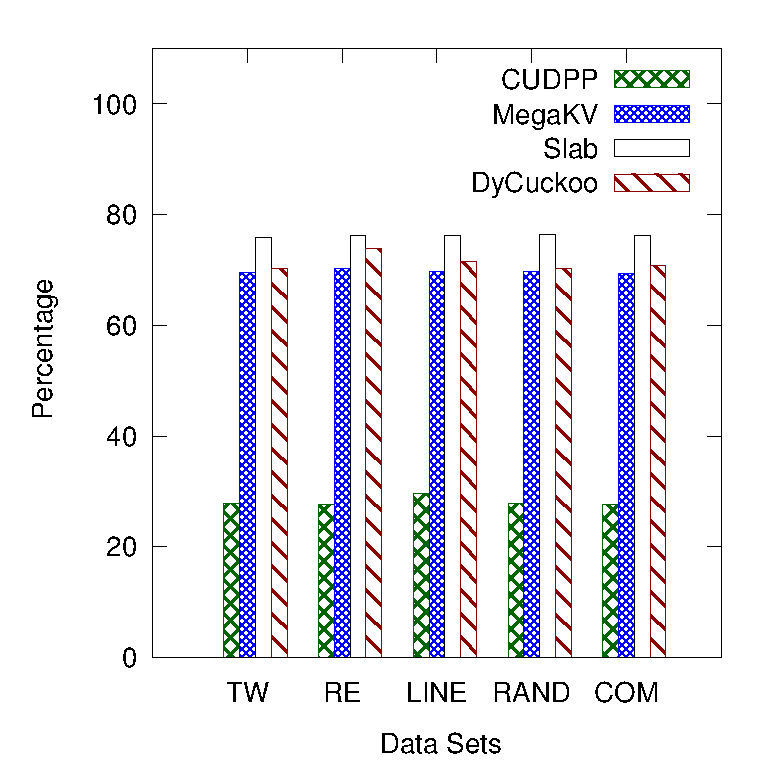
\includegraphics[width=\linewidth]{pic/static-profi/warp.eps}
%		\centerline{Warp Efficiency}
%	\end{minipage}
%	\hfill
%	\begin{minipage}{0.3\linewidth}\centering
%		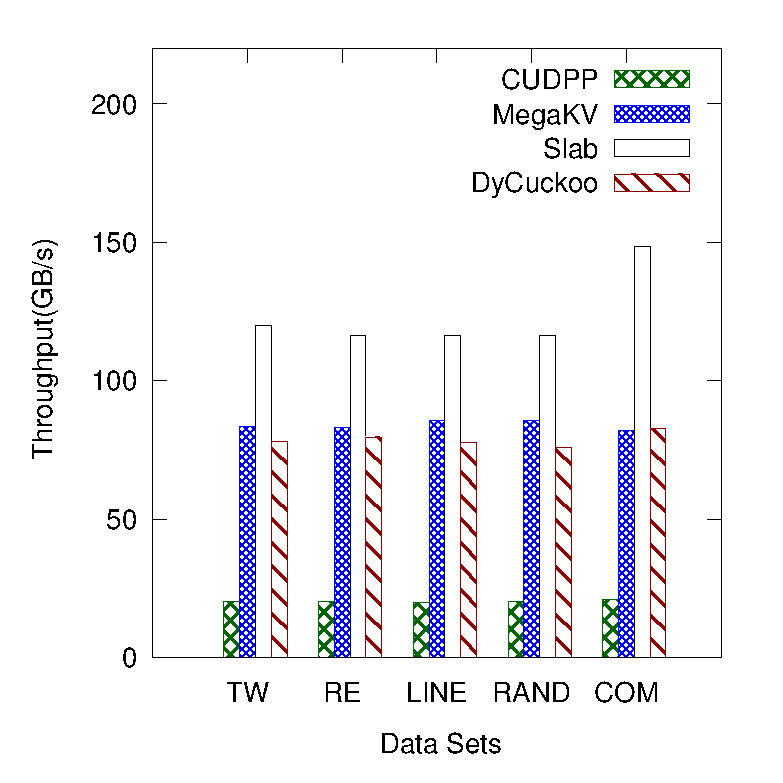
\includegraphics[width=\linewidth]{pic/static-profi/L2-read.eps}
%		\centerline{Cache Utilization}
%	\end{minipage}
%	\hfill
%	\begin{minipage}{0.3\linewidth}\centering
%		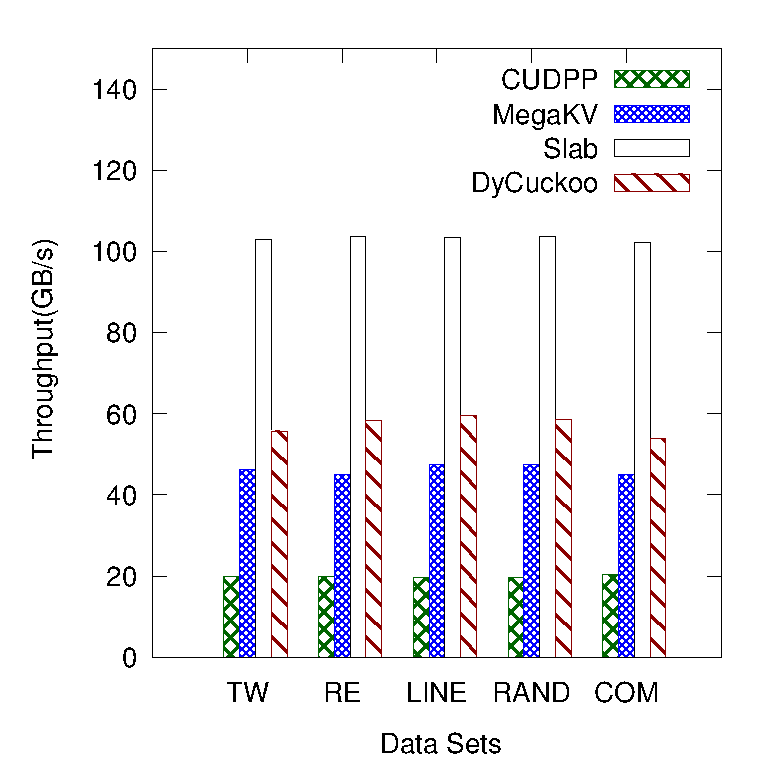
\includegraphics[width=\linewidth]{pic/static-profi/memory-read.eps}
%		\centerline{Memory Bandwidth Utilization}
%	\end{minipage}
%	\caption{GPU profiling results for static hashing comparison.}
%	\label{fig:static:profile}
%\end{figure*}


\vspace{1mm}\noindent\textbf{Dynamic Hashing Comparison (Section~\ref{sec:exp:dynamic}).}
Under the dynamic setting, we generate the workloads by batching the hash table operations. 
We partition the datasets into batches of $1$ million insertions. 
For each batch, we augment $1$ million \formal{find} operations and $1 \cdot r$ million \formal{delete} operations,
where $r$ is a parameter to balance insertions and deletions.
After we exhaust all the batches, we rerun these batches by swapping the \formal{insert} and \formal{delete} operations in each batch. 
We evaluate the performance of all compared approaches except \cudpp as it does not support deletions. 
Since \megakv is a static hash table, we double/half the memory usage followed by rehashing all KV pairs as its resizing strategy, if the corresponding filled factor falls out of the specified range. 
Moreover, if an insertion failure is found for a compared approach, we trigger its resizing strategy.

\begin{table}[t]
	\centering
	\caption{Parameters in the experiments}
	\vspace{-1.5em}
	\label{tbl:parameters}
	\begin{tabular}{|c|c|c|}
		\hline
		\textbf{Parameter} & \textbf{Settings} & \textbf{Default} \\ \hline
		Filled Factor	$\theta$  & 70\%, 75\%, 80\%, 85\%, 90\% & 85\% \\ \hline
		Lower Bound $\alpha$ & 20\%, 25\%, 30\%, 35\%, 40\% & 30\% \\ \hline
		Upper Bound	$\beta$  & 70\%, 75\%, 80\%, 85\%, 90\% & 85\% \\ \hline
		Ratio $r$ & 0.1, 0.2, 0.3, 0.4, 0.5 & 0.2 \\ \hline
		Batch Size & 2e5, 4e5, 6e5, 8e5, 10e5 & 10e5 \\ \hline
	\end{tabular}
\end{table}

\vspace{1mm}\noindent\textbf{Parameters.}
We vary the parameters when comparing \voter with the baselines.
$\alpha$ is the lower bound on the filled factor $\theta$ for all compared approaches,
whereas $\beta$ is the respective upper bound.
$r$ is the ratio of insertions over deletions in a processing batch. 
The settings of the aforementioned parameters could be found in Table~\ref{tbl:parameters}. For all experiments, we use \emph{million operations/seconds} (Mops) to measure the performance of all compared approaches.

\vspace{1mm}\noindent\textbf{Experiment Environment.}
We conduct all experiments on an Intel Xeon E5-2620 Server equipped with NVIDIA GeForce GTX 1080.The GTX 1080 is built on Pascal architecture with 20 SMs and 128 SPs per SM. The GTX 1080 has 8 GB of GDDR5 memory. Evaluations are performed using CUDA 9.1 on Ubuntu 16.04.3. The optimization level (-O3) is applied for compiling all programs.



\begin{figure}[t]
	\begin{minipage}{0.48\linewidth}\centering
		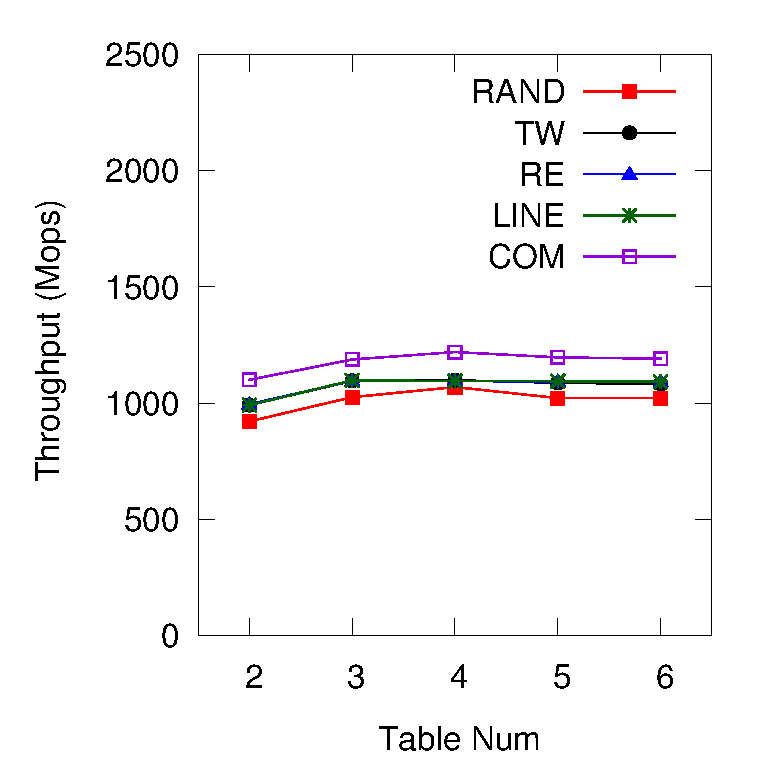
\includegraphics[width=\linewidth]{pic/tunning/tunning-insert.eps}
		\centerline{\formal{insert}}
	\end{minipage}
	\hfill
	\begin{minipage}{0.48\linewidth}\centering
		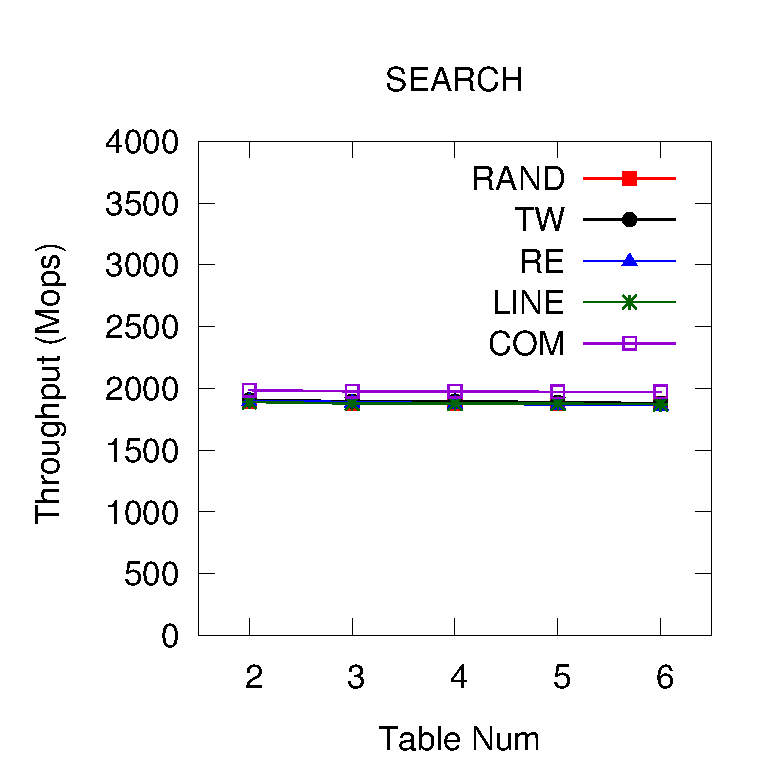
\includegraphics[width=\linewidth]{pic/tunning/tunning-search.eps}
		\centerline{\formal{find}}
	\end{minipage}
	\caption{Throughput of \voter for varying the number of hash tables.}
	\label{fig:vary-table}
\end{figure}
%
\begin{figure}[t]
	\begin{minipage}{0.48\linewidth}\centering
		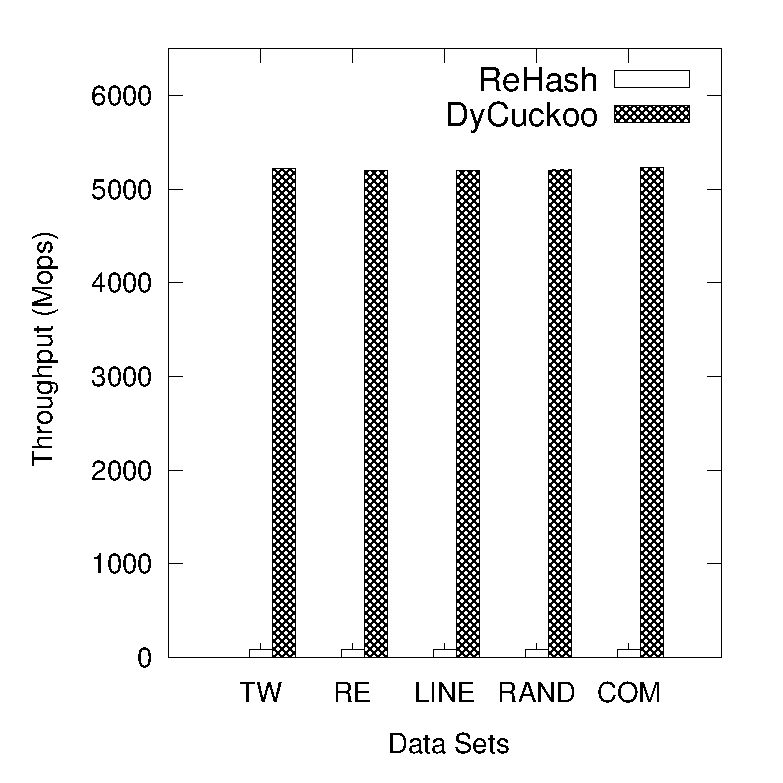
\includegraphics[width=\linewidth]{pic/compare/upsize.eps}
		\centerline{\formal{upsize}}
	\end{minipage}
	\hfill
	\begin{minipage}{0.48\linewidth}\centering
		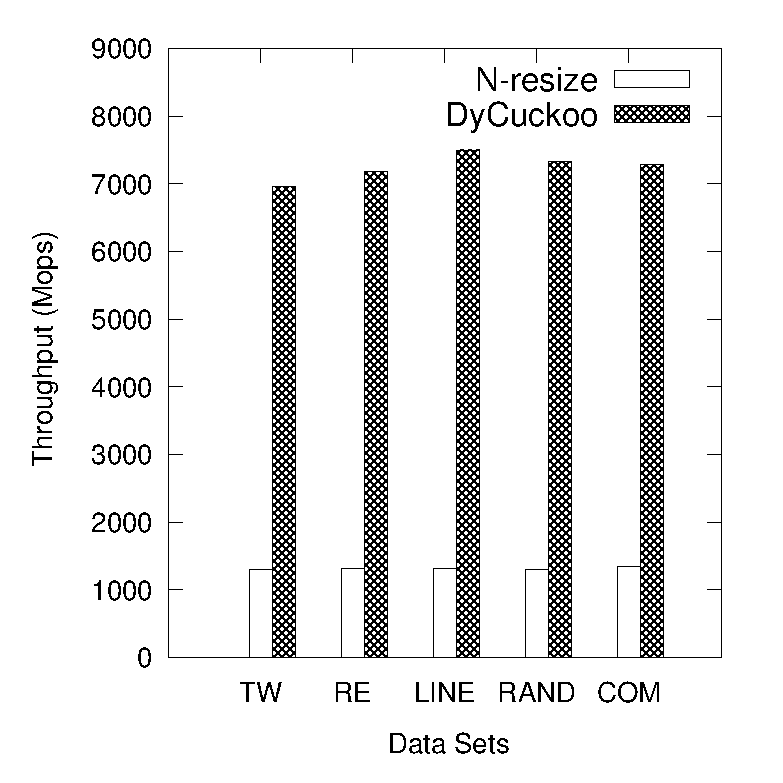
\includegraphics[width=\linewidth]{pic/compare/downsize.eps}
		\centerline{\formal{downsize}}
	\end{minipage}
	\caption{Throughput of subtable resize.}
	\label{fig:resize}
\end{figure}

\subsection{Sensitivity Analysis}\label{sec:exp:tune}

\vspace{1mm}
\noindent\textbf{Vary the number of tables.}
A key parameter that affects the performance of \voter is the number of hash table chosen. For the static scenario, we present the throughput performance of \formal{insert} and \formal{find} for varying number of hash tables in Figure~\ref{fig:vary-table}, while fixing the memory space of the entire structure to ensure the default filled factor $\theta$. 
The throughput of \formal{insert} increases with more hash tables, since there are more alternative locations for relocating a KV pair. However, the marginal improvement drops slightly for a larger number of hash tables. Furthermore, the throughput of \formal{find} remains constant for additional hash tables as the two-layer cuckoo hashing guarantees at most two look ups for \formal{find}. In the remaining part of this section, we fix the number of hash tables to be $4$.

\vspace{1mm}
\noindent\textbf{Resizing analysis.}
To validate the effectiveness of our resizing strategy proposed in Section~\ref{sec:dyn}, we compare it with rehashing. 
For evaluating upsizing, we initialize \voter with all the data and the filled factor as the default upper bound $85\%$. Then, we perform one time upsizing, i.e., upsize one subtable, and compare our resizing strategy against rehashing all the entries in the subtable by reinserting the entries with Algorithm~\ref{algo:insert}.
For evaluating downsizing, the setup is a mirror image of the upsizing evaluation with an initializing filled factor as the default lower bound $30\%$. 
The throughputs are reported in Figure~\ref{fig:resize}. 
The throughput of rehashing for the upsizing scenario is severely limited, since the remaining subtables not being upsized are almost filled and inserting KV pairs resulting frequent evictions.  
In comparison, the downsizing throughput of rehashing is significantly faster due to a low filled ratio.
Our resizing strategy achieves dramatic speedups over rehashing for downsizing as well. Besides, it only locks the subtable being resized and supports concurrent updates for the remaining subtables. 

\begin{figure}[t]
	\begin{minipage}{0.48\linewidth}\centering
		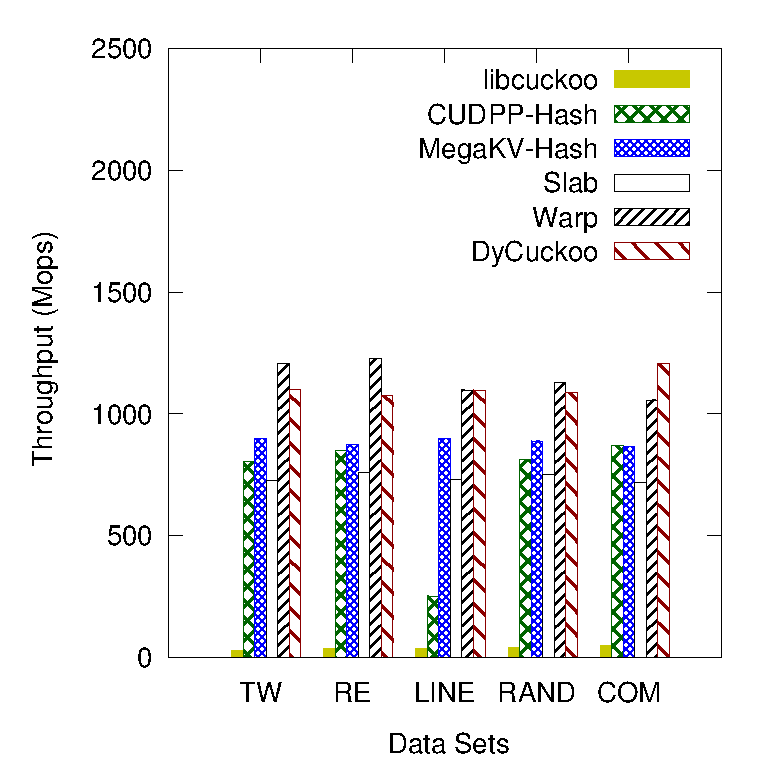
\includegraphics[width=\linewidth]{pic/static/static_insert.eps}
		\centerline{\formal{insert}}
	\end{minipage}
	\hfill
	\begin{minipage}{0.48\linewidth}\centering
		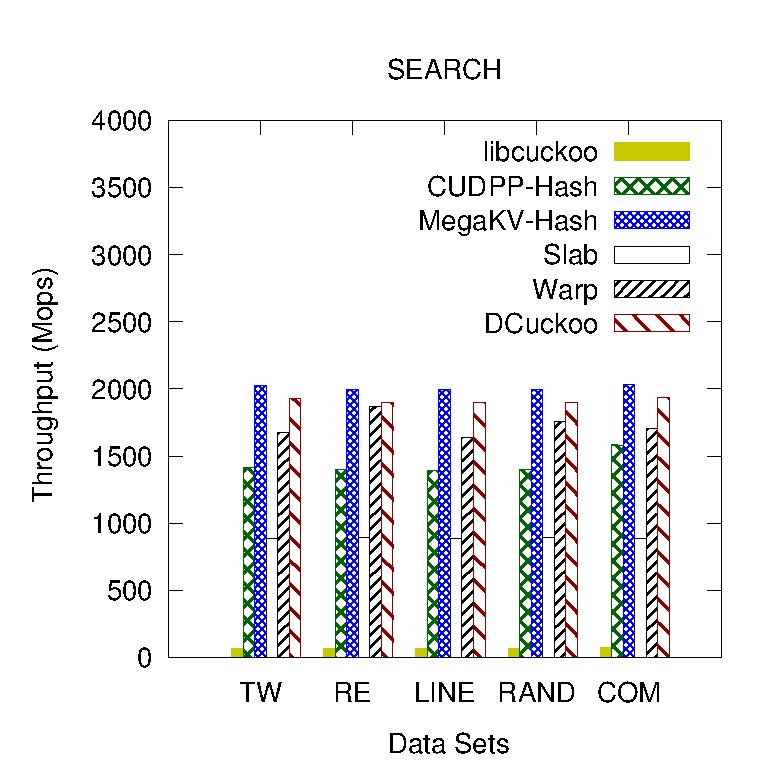
\includegraphics[width=\linewidth]{pic/static/static_search.eps}
		\centerline{\formal{find}}
	\end{minipage}
	\caption{Throughput of all compared approaches under the static setting.}
	\label{fig:static-all}
\end{figure}
%
\begin{figure}[t]
	\begin{minipage}{0.48\linewidth}\centering
		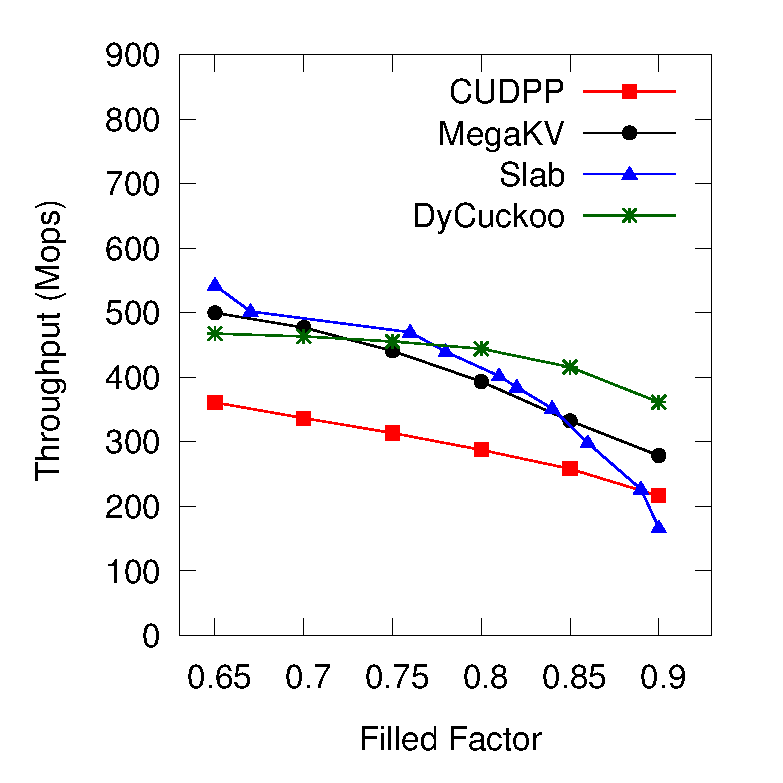
\includegraphics[width=\linewidth]{pic/static-load_factor/insert.eps}
		\centerline{\formal{insert}}
	\end{minipage}
	\hfill
	\begin{minipage}{0.48\linewidth}\centering
		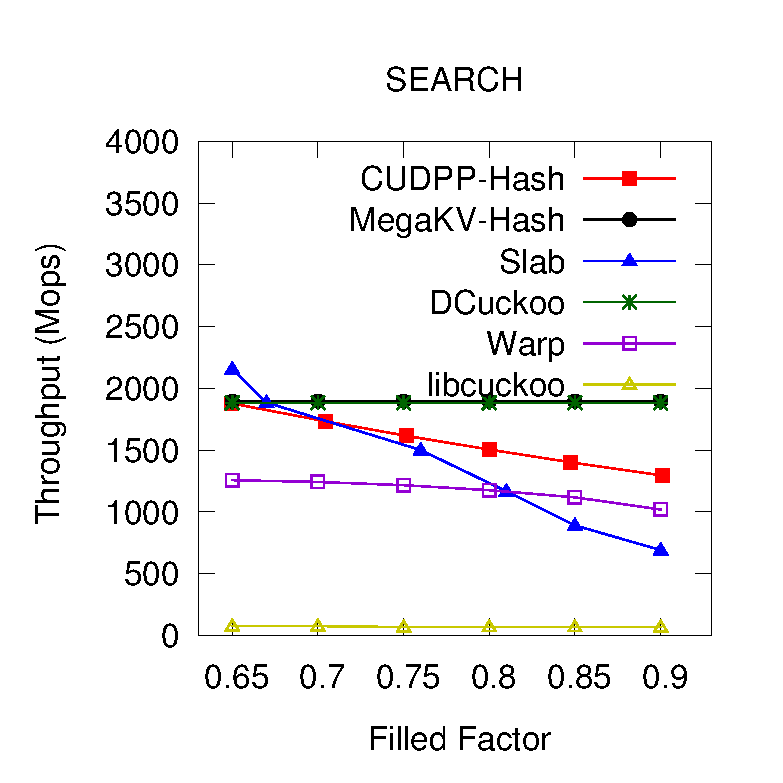
\includegraphics[width=\linewidth]{pic/static-load_factor/search.eps}
		\centerline{\formal{find}}
	\end{minipage}
	\caption{Throughput of all compared approaches for varying the filled factor against the \dsrandom dataset.}
	\label{fig:static-filled-factor}
\end{figure}

\begin{figure*}[htp]
	\begin{minipage}{0.19\linewidth}\centering
		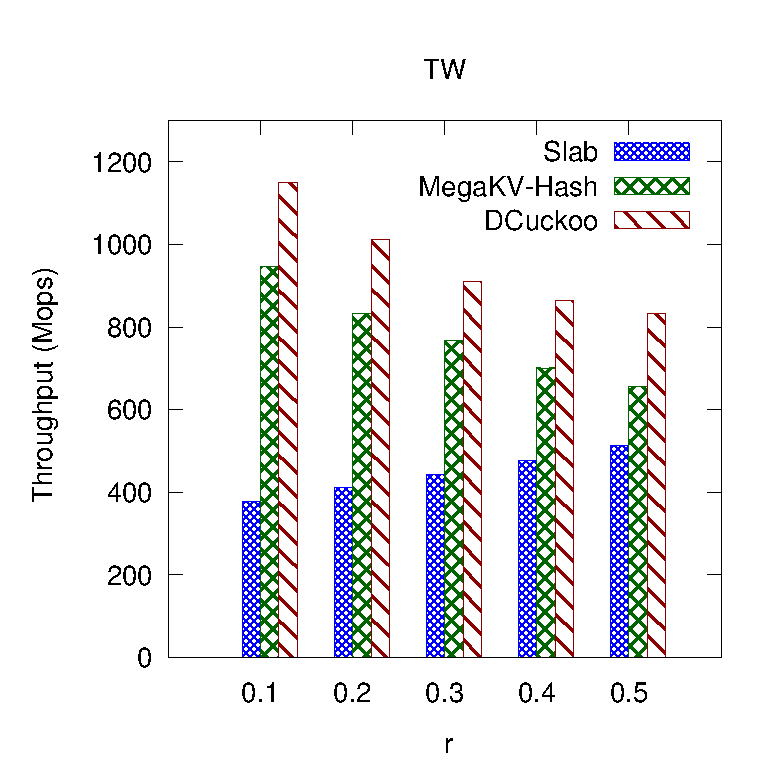
\includegraphics[width=\linewidth]{pic/dynamic/r/dynamic_twitter.eps}
		\centerline{\dstwitter}
	\end{minipage}
	\begin{minipage}{0.19\linewidth}\centering
		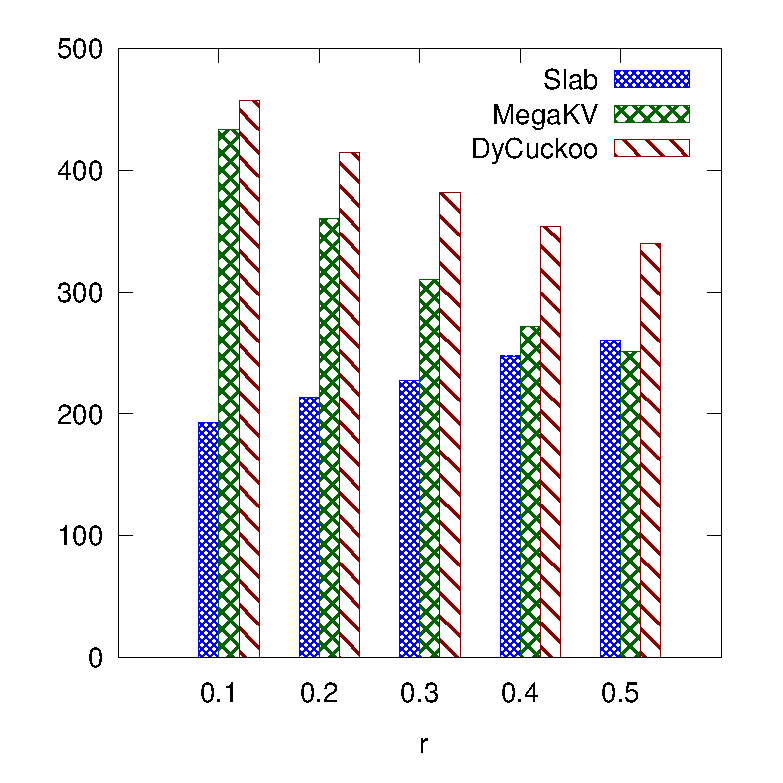
\includegraphics[width=\linewidth]{pic/dynamic/r/dynamic_reddit.eps}
		\centerline{\dsreddit}
	\end{minipage}
	\begin{minipage}{0.19\linewidth}\centering
		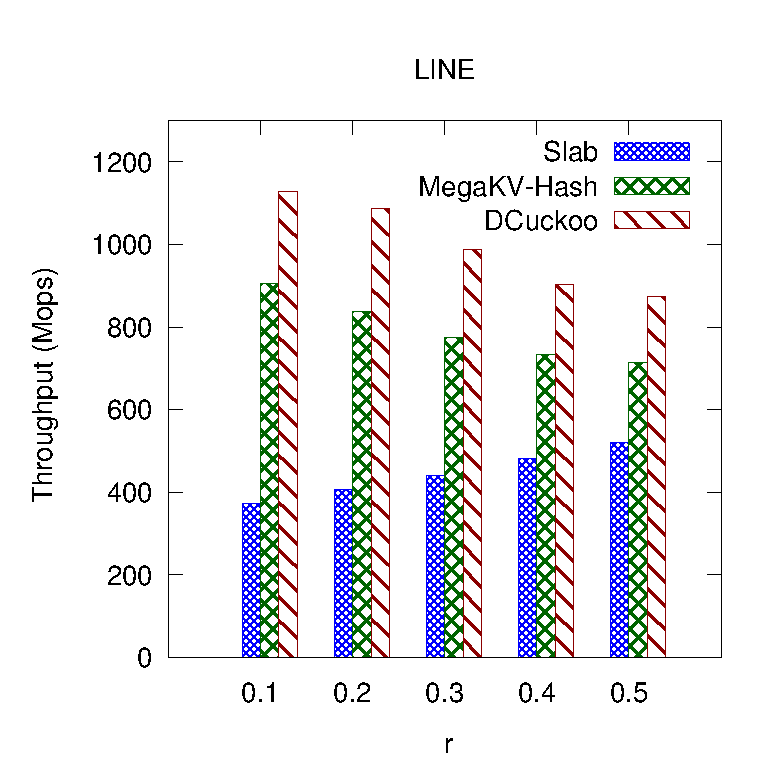
\includegraphics[width=\linewidth]{pic/dynamic/r/dynamic_tpch.eps}
		\centerline{\dstpch}
	\end{minipage}
	\begin{minipage}{0.19\linewidth}\centering
		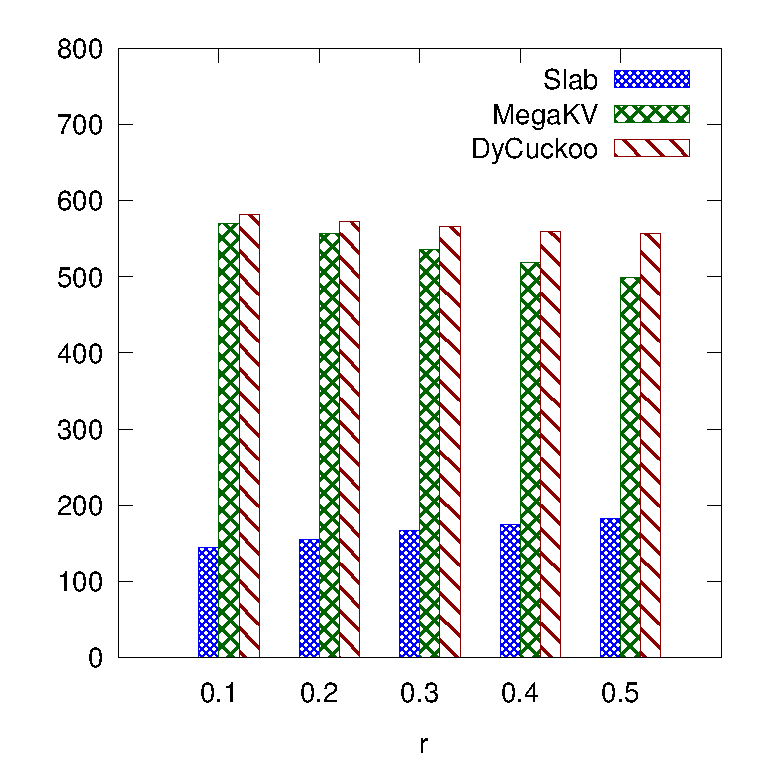
\includegraphics[width=\linewidth]{pic/dynamic/r/dynamic_ali.eps}
		\centerline{\dsali}
	\end{minipage}
	\begin{minipage}{0.19\linewidth}\centering
		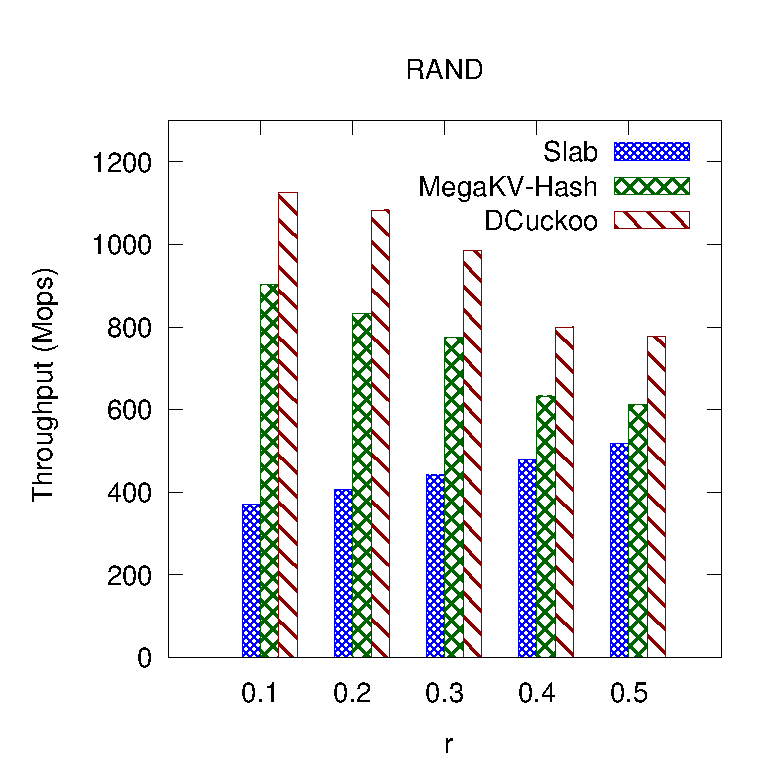
\includegraphics[width=\linewidth]{pic/dynamic/r/dynamic_random.eps}
		\centerline{\dsrandom}
	\end{minipage}
	\caption{Throughput for varying the ratio $r$.}
	\label{fig:vary-r-time}
\end{figure*}
%
\begin{figure*}[htp]
	\begin{minipage}{0.19\linewidth}\centering
		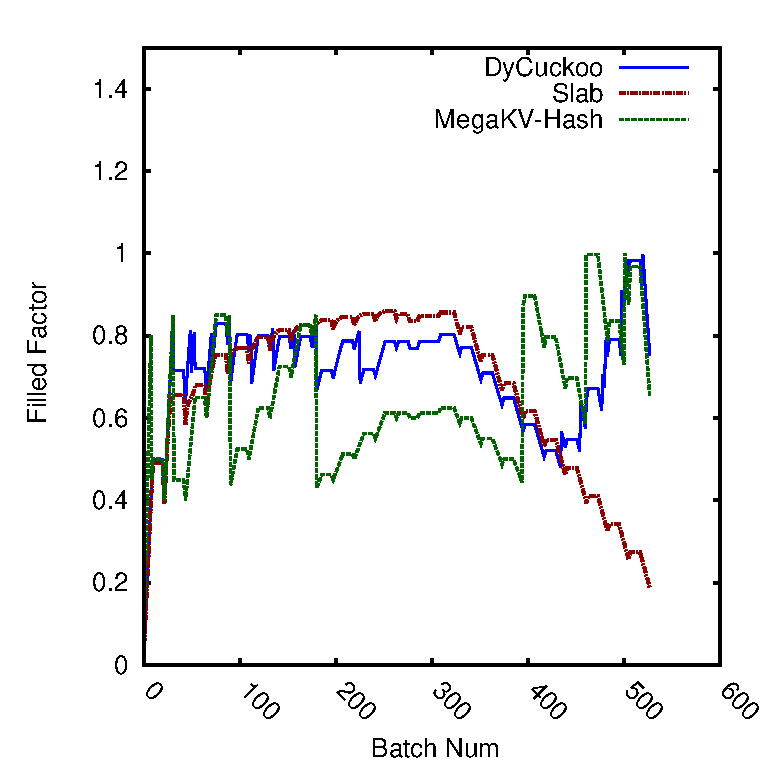
\includegraphics[width=\linewidth]{pic/dynamic-load_factor/twitter/batch_LoadFactor-2.eps}
		\centerline{\dstwitter}
	\end{minipage}
	\begin{minipage}{0.19\linewidth}\centering
		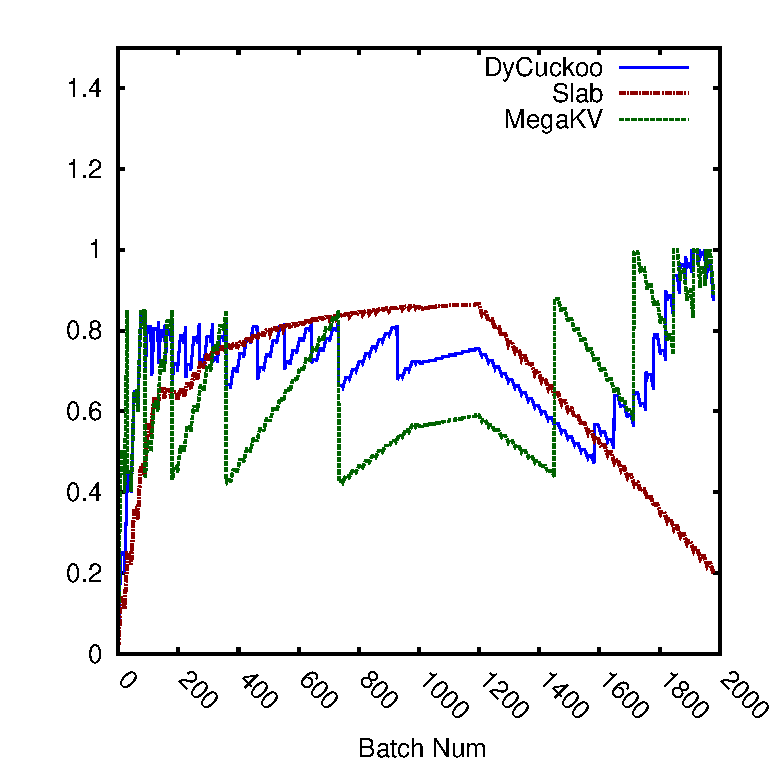
\includegraphics[width=\linewidth]{pic/dynamic-load_factor/reddit/batch_LoadFactor-2.eps}
		\centerline{\dsreddit}
	\end{minipage}
	\begin{minipage}{0.19\linewidth}\centering
		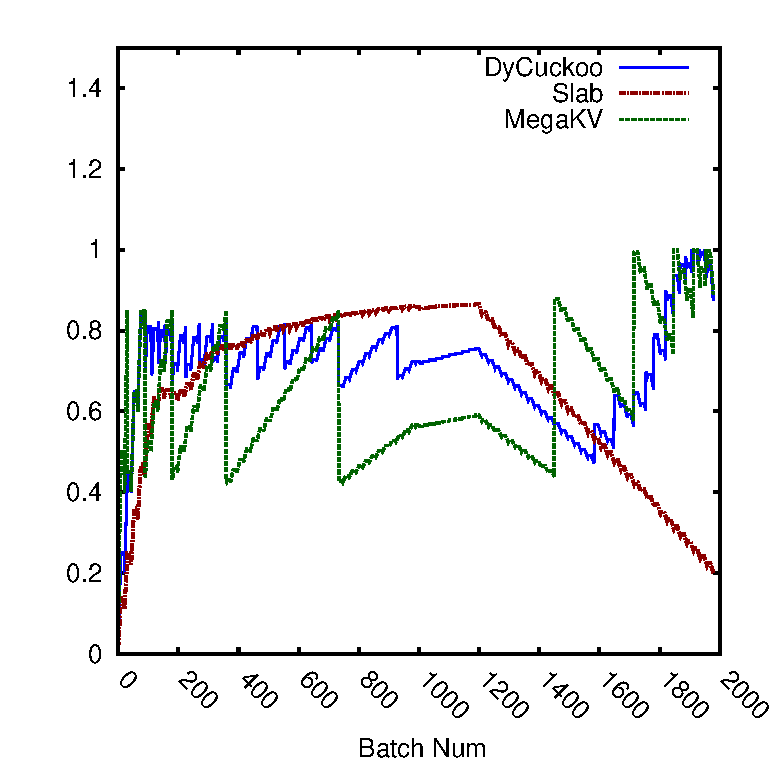
\includegraphics[width=\linewidth]{pic/dynamic-load_factor/tpch/batch_LoadFactor-2.eps}
		\centerline{\dstpch}
	\end{minipage}
	\begin{minipage}{0.19\linewidth}\centering
		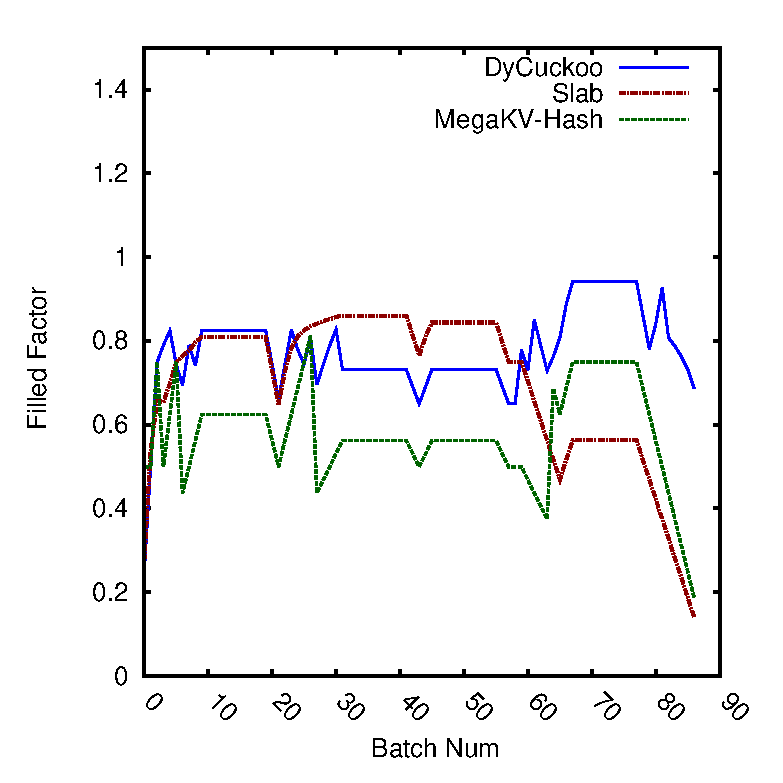
\includegraphics[width=\linewidth]{pic/dynamic-load_factor/ali/batch_LoadFactor-2.eps}
		\centerline{\dsali}
	\end{minipage}
	\begin{minipage}{0.19\linewidth}\centering
		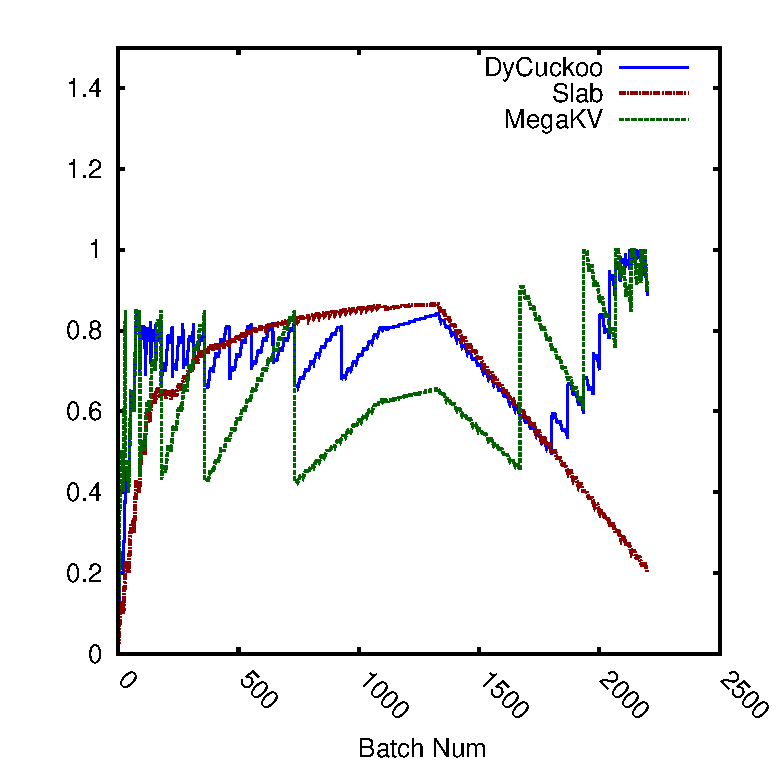
\includegraphics[width=\linewidth]{pic/dynamic-load_factor/random/batch_LoadFactor-2.eps}
		\centerline{\dsrandom}
	\end{minipage}
	\caption{Tracking the filled factor.}
	\label{fig:track-stability}
\end{figure*}
%
\begin{figure*}[htp]
	\begin{minipage}{0.19\linewidth}\centering
		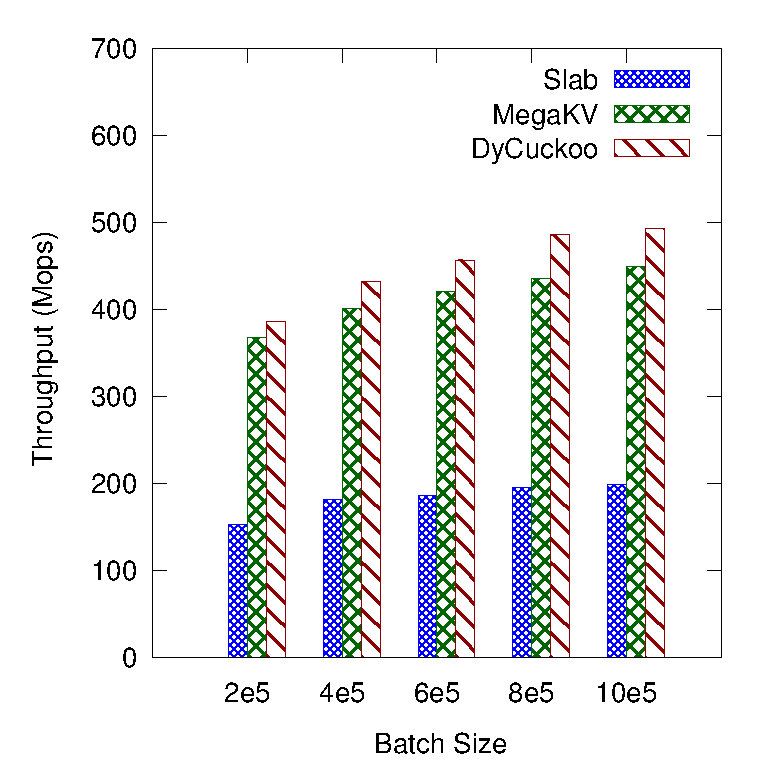
\includegraphics[width=\linewidth]{pic/dynamic/batch/dynamic_twitter.eps}
		\centerline{\dstwitter}
	\end{minipage}
	\begin{minipage}{0.19\linewidth}\centering
		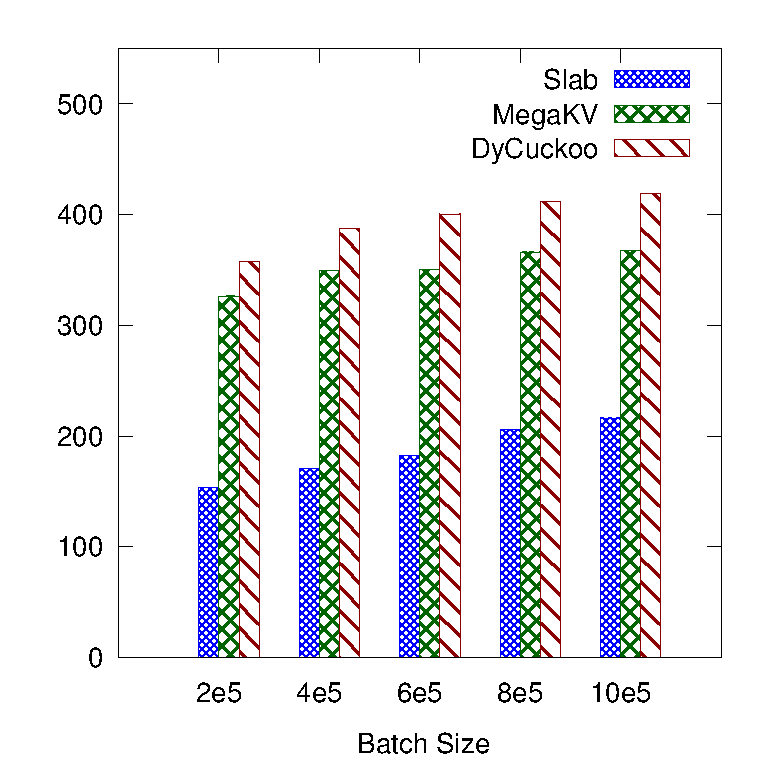
\includegraphics[width=\linewidth]{pic/dynamic/batch/dynamic_reddit.eps}
		\centerline{\dsreddit}
	\end{minipage}
	\begin{minipage}{0.19\linewidth}\centering
		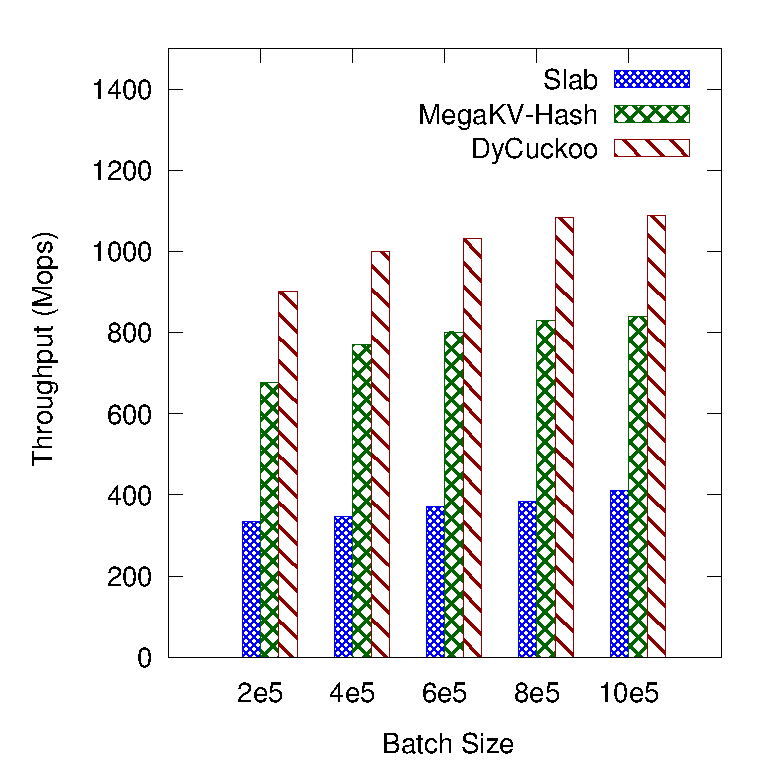
\includegraphics[width=\linewidth]{pic/dynamic/batch/dynamic_tpch.eps}
		\centerline{\dstpch}
	\end{minipage}
	\begin{minipage}{0.19\linewidth}\centering
		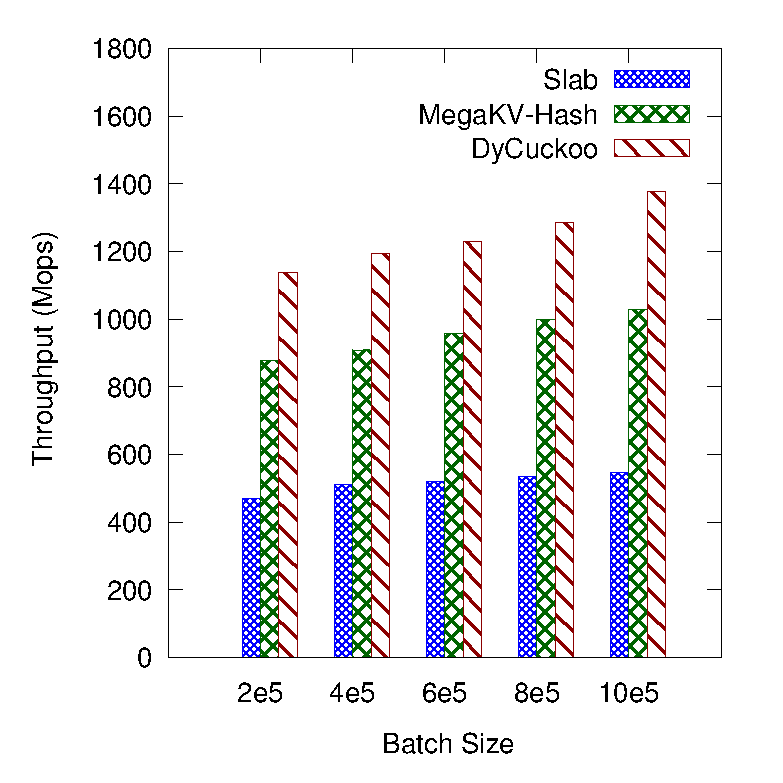
\includegraphics[width=\linewidth]{pic/dynamic/batch/dynamic_ali.eps}
		\centerline{\dsali}
	\end{minipage}
	\begin{minipage}{0.19\linewidth}\centering
		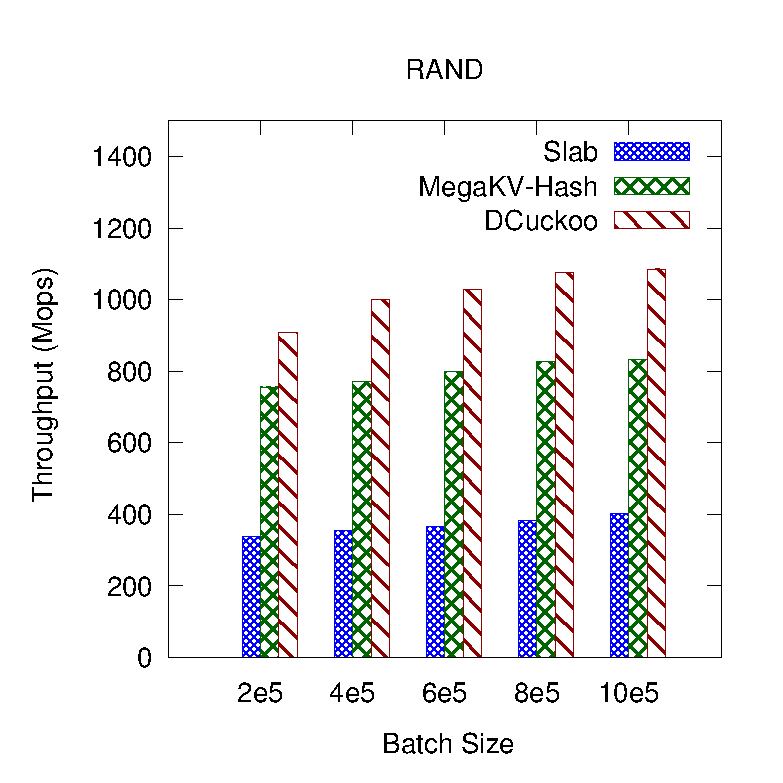
\includegraphics[width=\linewidth]{pic/dynamic/batch/dynamic_random.eps}
		\centerline{\dsrandom}
	\end{minipage}
	\caption{Throughput for varying Batch Size .}
	\label{fig:vary-batch-size}
\end{figure*}

\subsection{Static Hashing Comparison}\label{sec:exp:static}

\vspace{1mm}\noindent\textbf{Throughput Analysis.} In Figure~\ref{fig:static-all}, we present the throughput of all compared approaches over all datasets under the default setting.
Both \megakv and \cudpp are cuckoo hash approaches but \megakv shows better performance due to its bucket structure, which fully utilizes the cache line for optimizing random access performance.
\megakv and \slab are competitive against each other
while our proposed \voter demonstrates the best throughput for insertion. This is because \voter can reallocate KV pairs to more buckets among $d$ hash tables whereas \megakv can only choose one of two buckets for a KV pair, which causes \megakv to have more evictions. For \formal{find}, \megakv shows the best performance since it simply checks two buckets for locating a KV pair.
Although \voter also checks two buckets, it has slightly inferior performance than \megakv as \voter employs another layer of hashing that adds cost to the overall performance. 
As \slab employs a chaining approach, it requires more random accesses to locate a KV pair along the chain when a high filled factor is required. Hence, \slab has inferior performance than those of \megakv and \voter.
The experiments show that \voter is competitive even for the static scenario.

\vspace{1mm}\noindent\textbf{Varying filled factor $\theta$.}
We vary the filled factor $\theta$ and show the performance of all compared approaches against the \dsrandom dataset. The other datasets show similar trend and thus we omit the results in the paper.
For cuckoo hash approaches, i.e., \cudpp, \megakv and \voter, 
the insertion performance slightly degrades for a higher filled factor. \voter shows better stability for insertion as it employs the two-layer hashing approach which allows it to reallocate KV pairs efficiently even when the hash table is almost filled ($\theta=90\%$).
As cuckoo hash approaches only require constant lookups for \formal{find}, the performance is not affected by the filled factor except \cudpp.
This is because \cudpp automatically chooses the number of hash functions given the data to be inserted (up to 5). 
Hence, it may employ more hash functions for higher filled factor to improve the insertion performance. 
However, this affects the throughput for \formal{find} as it needs to check more locations to get one KY pair.  
For \slab, the performance of both \formal{insert} and \formal{find} is dramatically affected by the filled factor. When $\theta=90\%$, \voter outperforms \slab by over 2x and 2.5x for \formal{insert} and \formal{find} respectively.


%\vspace{1mm}\noindent\textbf{GPU Profiling.} To further study the behavior of the approaches, we present three types of profiling results for all \formal{insert} GPU kernels in Figure~\ref{fig:static:profile}.
%For \emph{warp efficiency}, \voter maintains a stable rate at around 70\%, which is significantly higher than the other two cuckoo hash approaches: \megakv and \cudpp.  
%We attribute this phenomenon to the voter mechanism proposed in Section~\ref{sec:vot:con}, which yields better overall load balancing. 
%\linear could achieve higher warp efficiency than \voter, but is very volatile across different datasets. This is because each \formal{insert} in \linear may require scanning varying number of hash values for distinct data distributions. 
%For example, in the \dsali dataset, its warp efficiency drops below 40\% since \dsali contains more duplicated keys than other datasets. 

%Looking at \emph{cache} and \emph{memory bandwidth} profiling results, \megakv and \voter demonstrate better utilization as they employ the bucket mechanism.
%As \voter always needs to use atomicCAS to lock a bucket before accessing it, its utilization is inferior than that of \megakv due to the additional IO when inserting a KV pair to a bucket. In addition, atomicCAS is less efficient than atomicExch as it involves more workload per operation (see Table~\ref{fig:atomic}). Nevertheless, implementations based on atomicExch only supports KV pair with 64 bits, whereas adopting atomicCAS in \voter can support arbitrary length as we lock the bucket for exclusive update.
%It is also noted that, even though \megakv has great cache utilization due to the use of atomicExch accessing buckets directly, the overall performance is eventually bounded by device memory IOs. 

%In summary, under the static environment, \voter achieves competitive efficiency against the compared GPU baselines. Moreover, although \voter does not deliver the best performance over existing approaches, it has very low insertion failure rate and supports more general hash tables.


%





\begin{figure*}[htp]
	\begin{minipage}{0.19\linewidth}\centering
		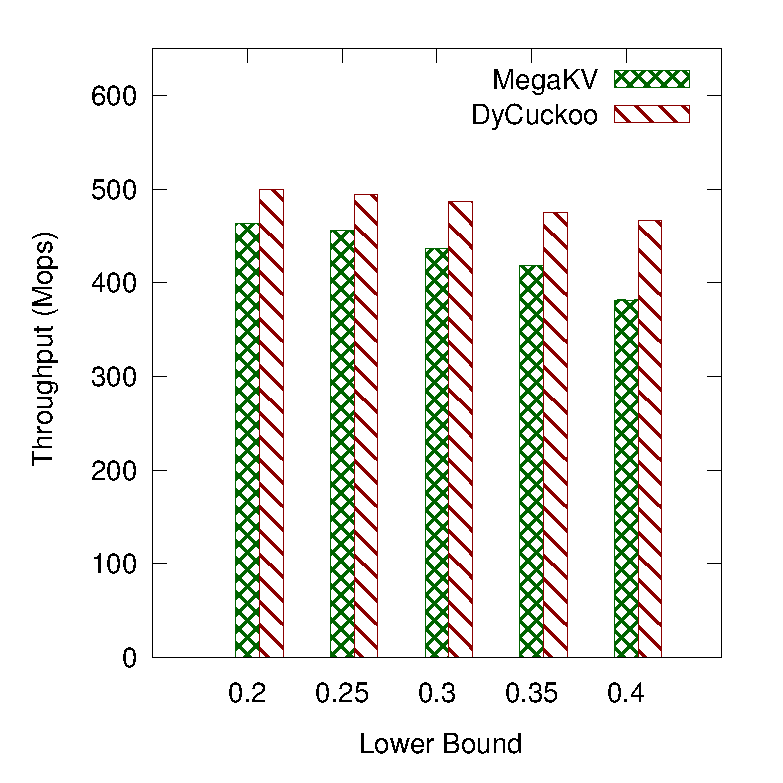
\includegraphics[width=\linewidth]{pic/dynamic/lower/dynamic_twitter.eps}
		\centerline{\dstwitter}
	\end{minipage}
	\begin{minipage}{0.19\linewidth}\centering
		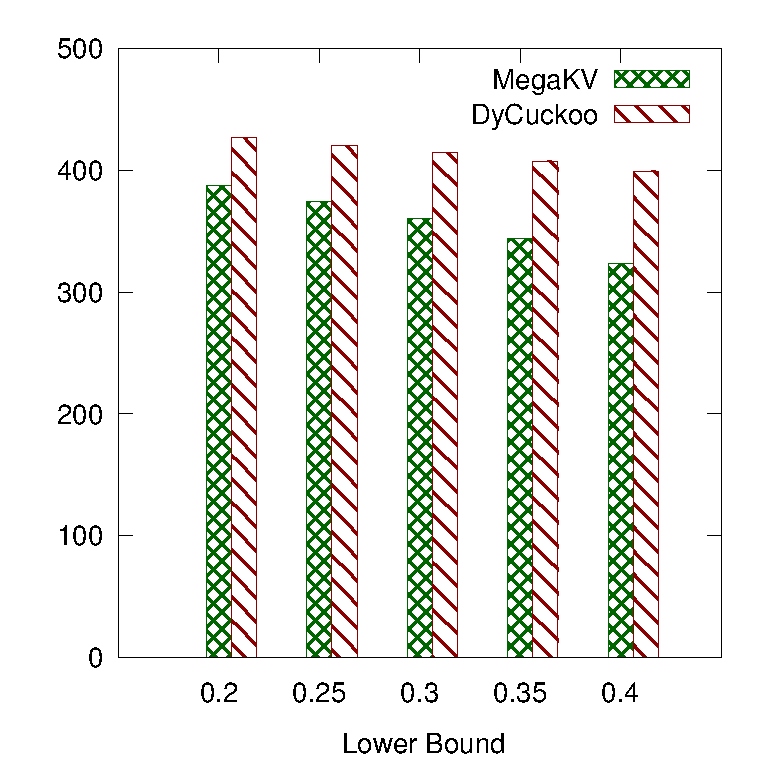
\includegraphics[width=\linewidth]{pic/dynamic/lower/dynamic_reddit.eps}
		\centerline{\dsreddit}
	\end{minipage}
	\begin{minipage}{0.19\linewidth}\centering
		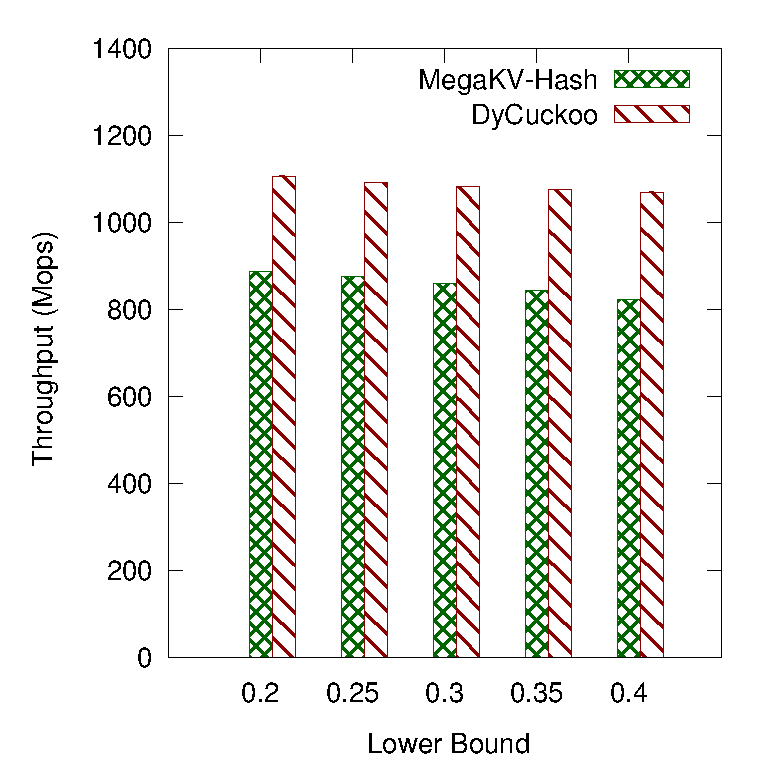
\includegraphics[width=\linewidth]{pic/dynamic/lower/dynamic_tpch.eps}
		\centerline{\dstpch}
	\end{minipage}
	\begin{minipage}{0.19\linewidth}\centering
		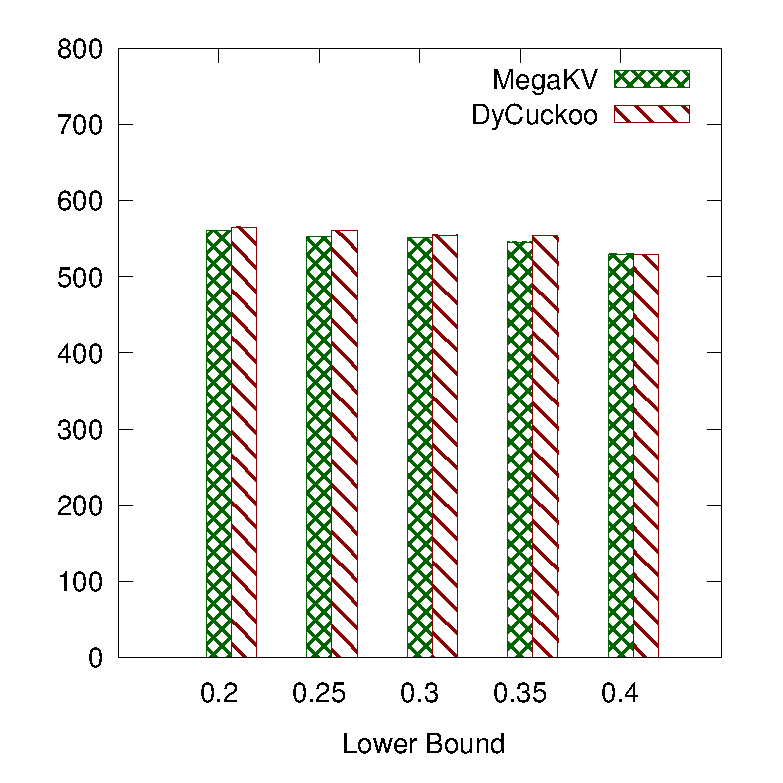
\includegraphics[width=\linewidth]{pic/dynamic/lower/dynamic_ali.eps}
		\centerline{\dsali}
	\end{minipage}
	\begin{minipage}{0.19\linewidth}\centering
		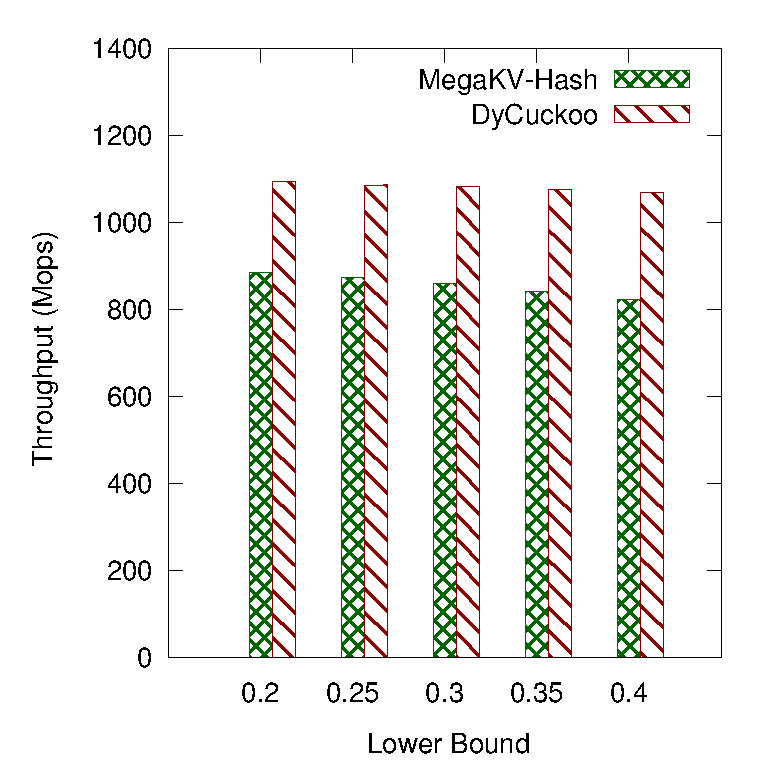
\includegraphics[width=\linewidth]{pic/dynamic/lower/dynamic_random.eps}
		\centerline{\dsrandom}
	\end{minipage}
	\caption{Throughput for varying $\alpha$ .}
	\label{fig:vary-lower-time}
\end{figure*}

\begin{figure*}[htp]
	\begin{minipage}{0.19\linewidth}\centering
		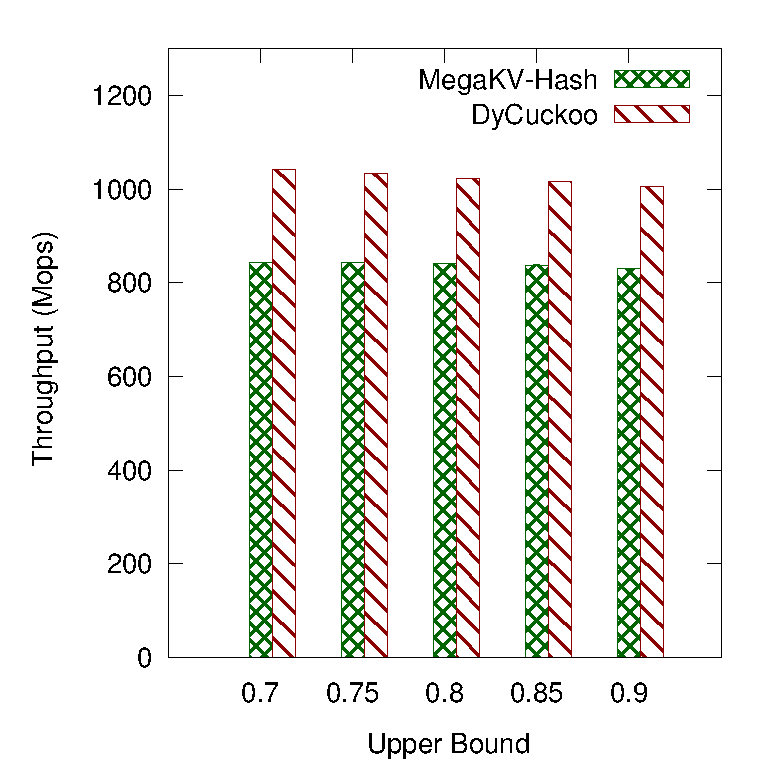
\includegraphics[width=\linewidth]{pic/dynamic/upper/dynamic_twitter.eps}
		\centerline{\dstwitter}
	\end{minipage}
	\begin{minipage}{0.19\linewidth}\centering
		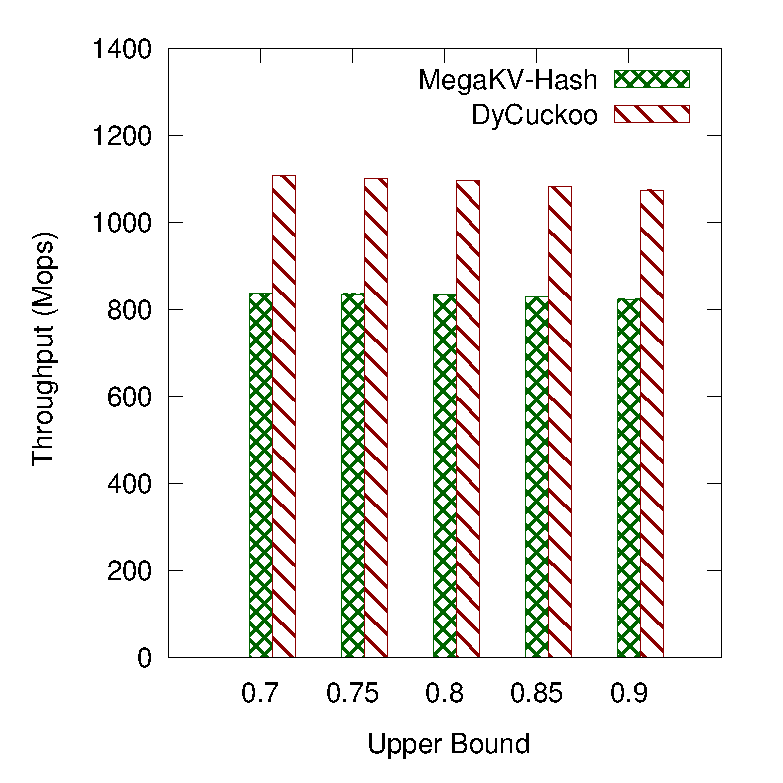
\includegraphics[width=\linewidth]{pic/dynamic/upper/dynamic_reddit.eps}
		\centerline{\dsreddit}
	\end{minipage}
	\begin{minipage}{0.19\linewidth}\centering
		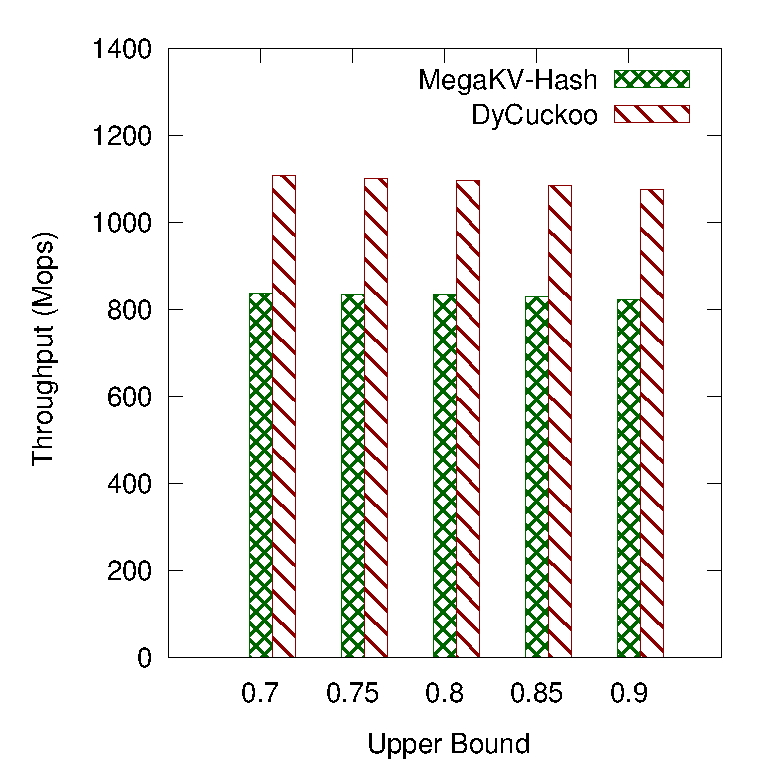
\includegraphics[width=\linewidth]{pic/dynamic/upper/dynamic_tpch.eps}
		\centerline{\dstpch}
	\end{minipage}
	\begin{minipage}{0.19\linewidth}\centering
		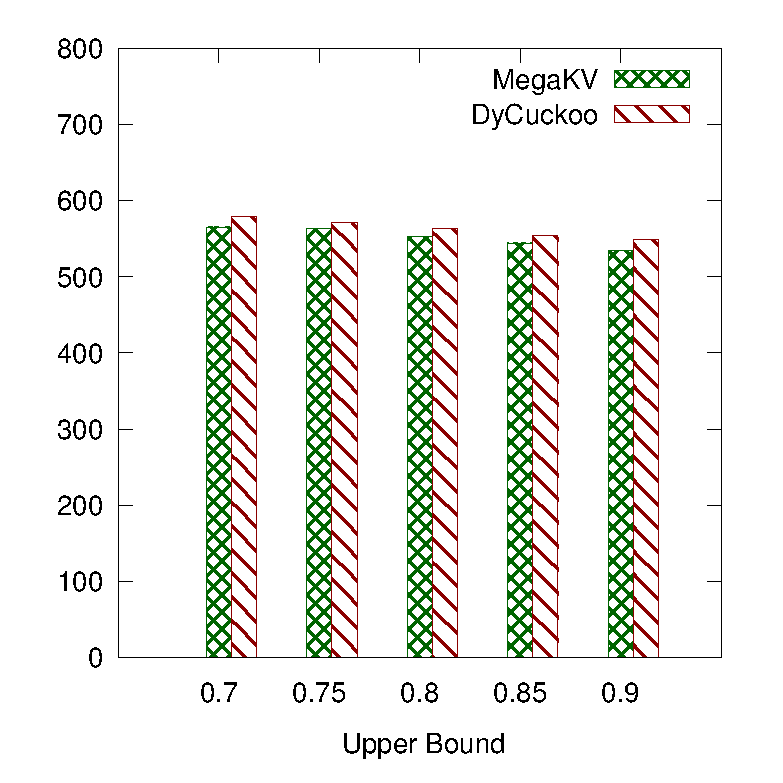
\includegraphics[width=\linewidth]{pic/dynamic/upper/dynamic_ali.eps}
		\centerline{\dsali}
	\end{minipage}
	\begin{minipage}{0.19\linewidth}\centering
		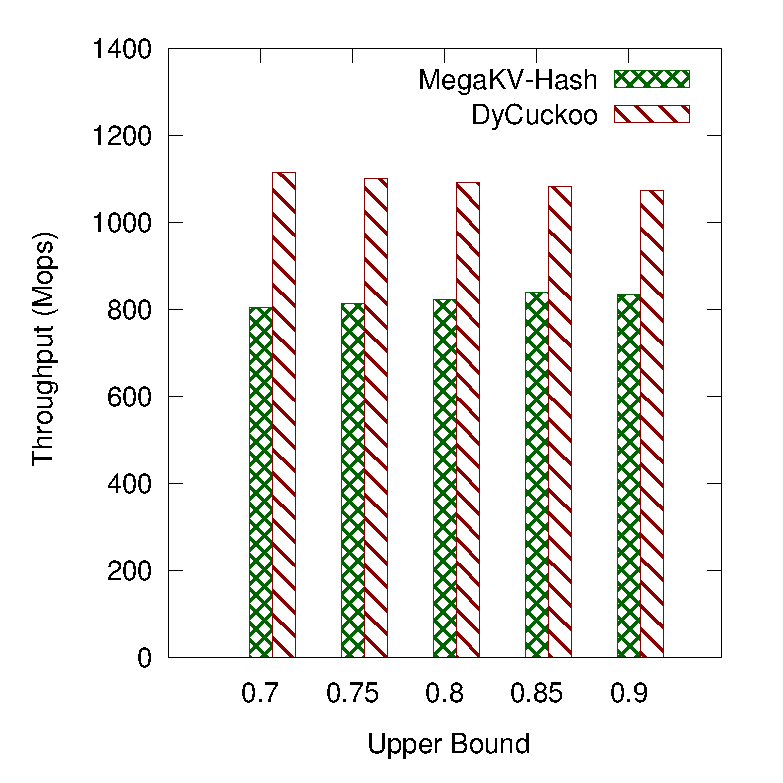
\includegraphics[width=\linewidth]{pic/dynamic/upper/dynamic_random.eps}
		\centerline{\dsrandom}
	\end{minipage}
	\caption{Throughput for varying $\beta$ .}
	\label{fig:vary-upper-time}
\end{figure*}

\subsection{Dynamic Hashing Comparison}\label{sec:exp:dynamic}

\noindent\textbf{Varying insert vs. delete ratio $r$.}
In Figure~\ref{fig:vary-r-time}, we report the results for varying the ratio $r$, i.e., number of deletions over number of insertions in a batch.
We have an interesting observation that, for a larger $r$, the performance of \voter and \megakv degrades whereas that of \slab improves. As a larger $r$ indicates more deletions, resizing operations are more frequently invoked for \voter and \megakv. In contrast, more deletions leads to additional vacant spaces for \slab as it simply symbolically marks a deleted KV pair. Insertions are processed more efficiently for \slab since the inserted KV pairs can overwrite the symbolically deleted ones. Hence, \slab utilizes more GPU device memory than \voter and \megakv. However, symbolic deletions cannot guarantee a bounded filled factor and may lead to arbitrary bad memory efficiency, which will be discussed with more experimental results later in this section.
\voter shows the best overall performance. Furthermore, the throughput margin between \voter and \megakv grows for a larger $r$. 
As aforementioned, larger $r$ triggers more resizing operations, where \voter is more efficient than \megakv since \megakv employs a total rehashing approach. 

%\linear and \megakv remains inefficient as they incur expensive overheads of resizing. An interesting observation for \linear and \megakv is that there exists a sweet spot where the resizing cost is the minimal.
%It is because the workload composition of insertions and deletions should be just right so that it does not trigger unnecessary upsizings or downsizings. However, in reality, the workloads could vary significantly and existing methods cannot be easily adapted while maintaining guaranteed filled factor. This has again validated the effectiveness of \voter against dynamic workloads.


\vspace{1mm}\noindent\textbf{Performance stability.}
We evaluate the performance stability of the compared approaches in Figure~\ref{fig:track-stability}. 
In particular, we track the filled factor after processing each batch.
\slab shows good stability in terms of memory usage for the starting phases. Unfortunately, due to the symbolic deletion approach employed, the memory efficiency of \slab degrades significantly as more deletions are processed. In particular, its filled factor drops to less than $20\%$ after processing less than 100 batches for the \dsali dataset, which deems for a complete rebuild.
%
\megakv shows unstable trend since it employs a simple double/half approach for resizing. We can see its filled factor jumps up or down dramatically at the points of resizing. \voter demonstrates the best overall stability and saves up to 4x memory over the compared baselines (the \dsali dataset). 
The results have validated our design where only one of the subtables are subject to resizing. 
Nevertheless, there is still rooms for improvement. We note that for some datasets, i.e., \dstwitter, \dsreddit, \dstpch and \dsrandom, we observe that the filled factor of \voter drops sharply.
This is because, even after one time of upsizing, the insertions fail due to too many evictions and it triggers another round of upsizing. We leave it as a future work. 


\vspace{1mm}\noindent\textbf{Varying the batch size.}
We have also varied the size of each processing batch. The results are reported in Figure~\ref{fig:vary-batch-size}. 
\slab remains to show inferior performance than \megakv and \voter. 
This is because \slab accommodates new inserted KV pairs with the chaining approach and does not increase the range of the unique hash values. Hence, a stream of insertions will eventually lead to long chains, which hurts the performance of hash table operations. Furthermore, \voter presents better performance than \megakv and the margin increases with a larger batch size.


\vspace{1mm}\noindent\textbf{Varying the filled factor lower bound $\alpha$.}
We vary the lower bound of the filled factor and report the results in Figure~\ref{fig:vary-lower-time}. 
We only compare \megakv and \voter since \slab is unable to control the filled factor because of \slab's symbolic deletion approach. 
Apparently, the simple resizing strategy adopted by \megakv incurs substantial overhead. Such overhead grows for a higher $\alpha$ since the number of downsizings increases. The performance of \voter is not affected significantly due to the incremental resizing approach by updating only one subtable at a time. We note that, the performance of \megakv is competitive against \voter for the \dsali dataset. This is because \megakv occupies significant more memory spaces than that of \voter, as evidenced in Figure~\ref{fig:track-stability} (up to 4x). Hence, \megakv trades space efficiency with time efficiency.
Nevertheless, \voter remains superior over \megakv in terms of time efficiency while saves GPU memory substantially. 



\vspace{1mm}\noindent\textbf{Varying the filled factor upper bound $\beta$.}
The results for varying $\beta$ is reported in Figure~\ref{fig:vary-upper-time}. 
It is interesting to see that the upper bound does not significantly affect the overall performance for \megakv and \voter. 
On one hand, higher filled factor leads to slower \formal{insert} performance. On the other hand, less number of rehashing incurred for a higher filled factor. Thus, the overall performance remains stable for both approaches as the opposing factors cancel each other. \megakv has competitive efficiency against \voter in the \dsali dataset. The reason is similar as we discussed for varying the lower bound $\alpha$.








\section{conclusion}\label{sec:con}
In this paper, we contribute a number of novel designs for dynamic hash table on GPUs. 
First, we introduced an efficient strategy to resize only one of a subtable at a time. Our theoretical analysis demonstrated the near-optimality of the resizing strategy. Second, we devised a two-layer cuckoo has scheme that ensures at most two loops for find and deletion operations, while still retains similar performance for insertion as general cuckoo hash tables. 
Empirically, our proposed design achieves competitive performance against the state-of-the-art static GPU hash tables. Our hash table design achieves superior performance while saves up to 4x memory over the state-of-the-art approaches against dynamic workloads.

 



%

\section*{Appendix}
We provide additional experiments for evaluating the static scenario performance when varying the filled factor. 
For \formal{insert}, the throughput of all approaches drops for a higher filled factor as it becomes harder to insert when the hash tables are almost filled.
For \formal{find}, all approaches except \linear has constant performance for different filled factor because they all fall into the category of cuckoo hash and has a fixed number of locations for lookups. 
Overall, \voter achieves the second best performance behind \megakv under the static scenario, which is consistent with our discussions in Section~\ref{sec:exp:static}.




%\pagebreak
\bibliographystyle{abbrv}
\bibliography{ref}

\begin{IEEEbiography}[{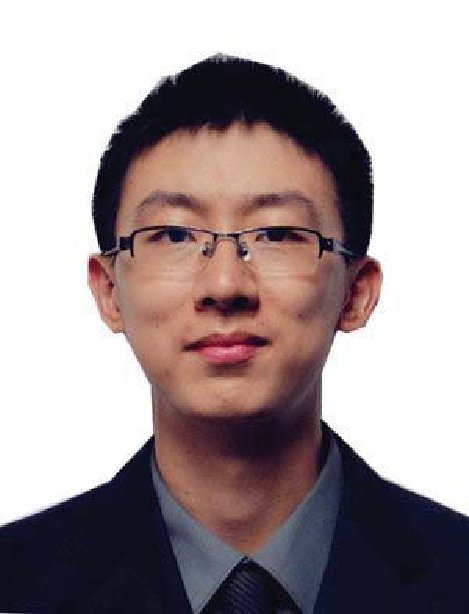
\includegraphics[width=1in,height=1.25in,clip,keepaspectratio]{photos/yuchen.pdf}}]
	{Yuchen Li} is an assistant professor at the School of Information Systems, Singapore Management University (SMU).
	%Before joining SMU, he was a research fellow in the School of Computing, National University of Singapore (NUS).
	He received the double B.Sc. degrees in applied math and computer science (both degrees with first class honors)
	and the Ph.D. degree in computer science from NUS, in 2013 and 2016, respectively. He received the Lee Kong Chian Fellowship in 2019 for research excellence.
	His research interests include heterogeneous computing, graph analytics and computational journalism.
\end{IEEEbiography}
\vspace*{-2\baselineskip}

\begin{IEEEbiography}[{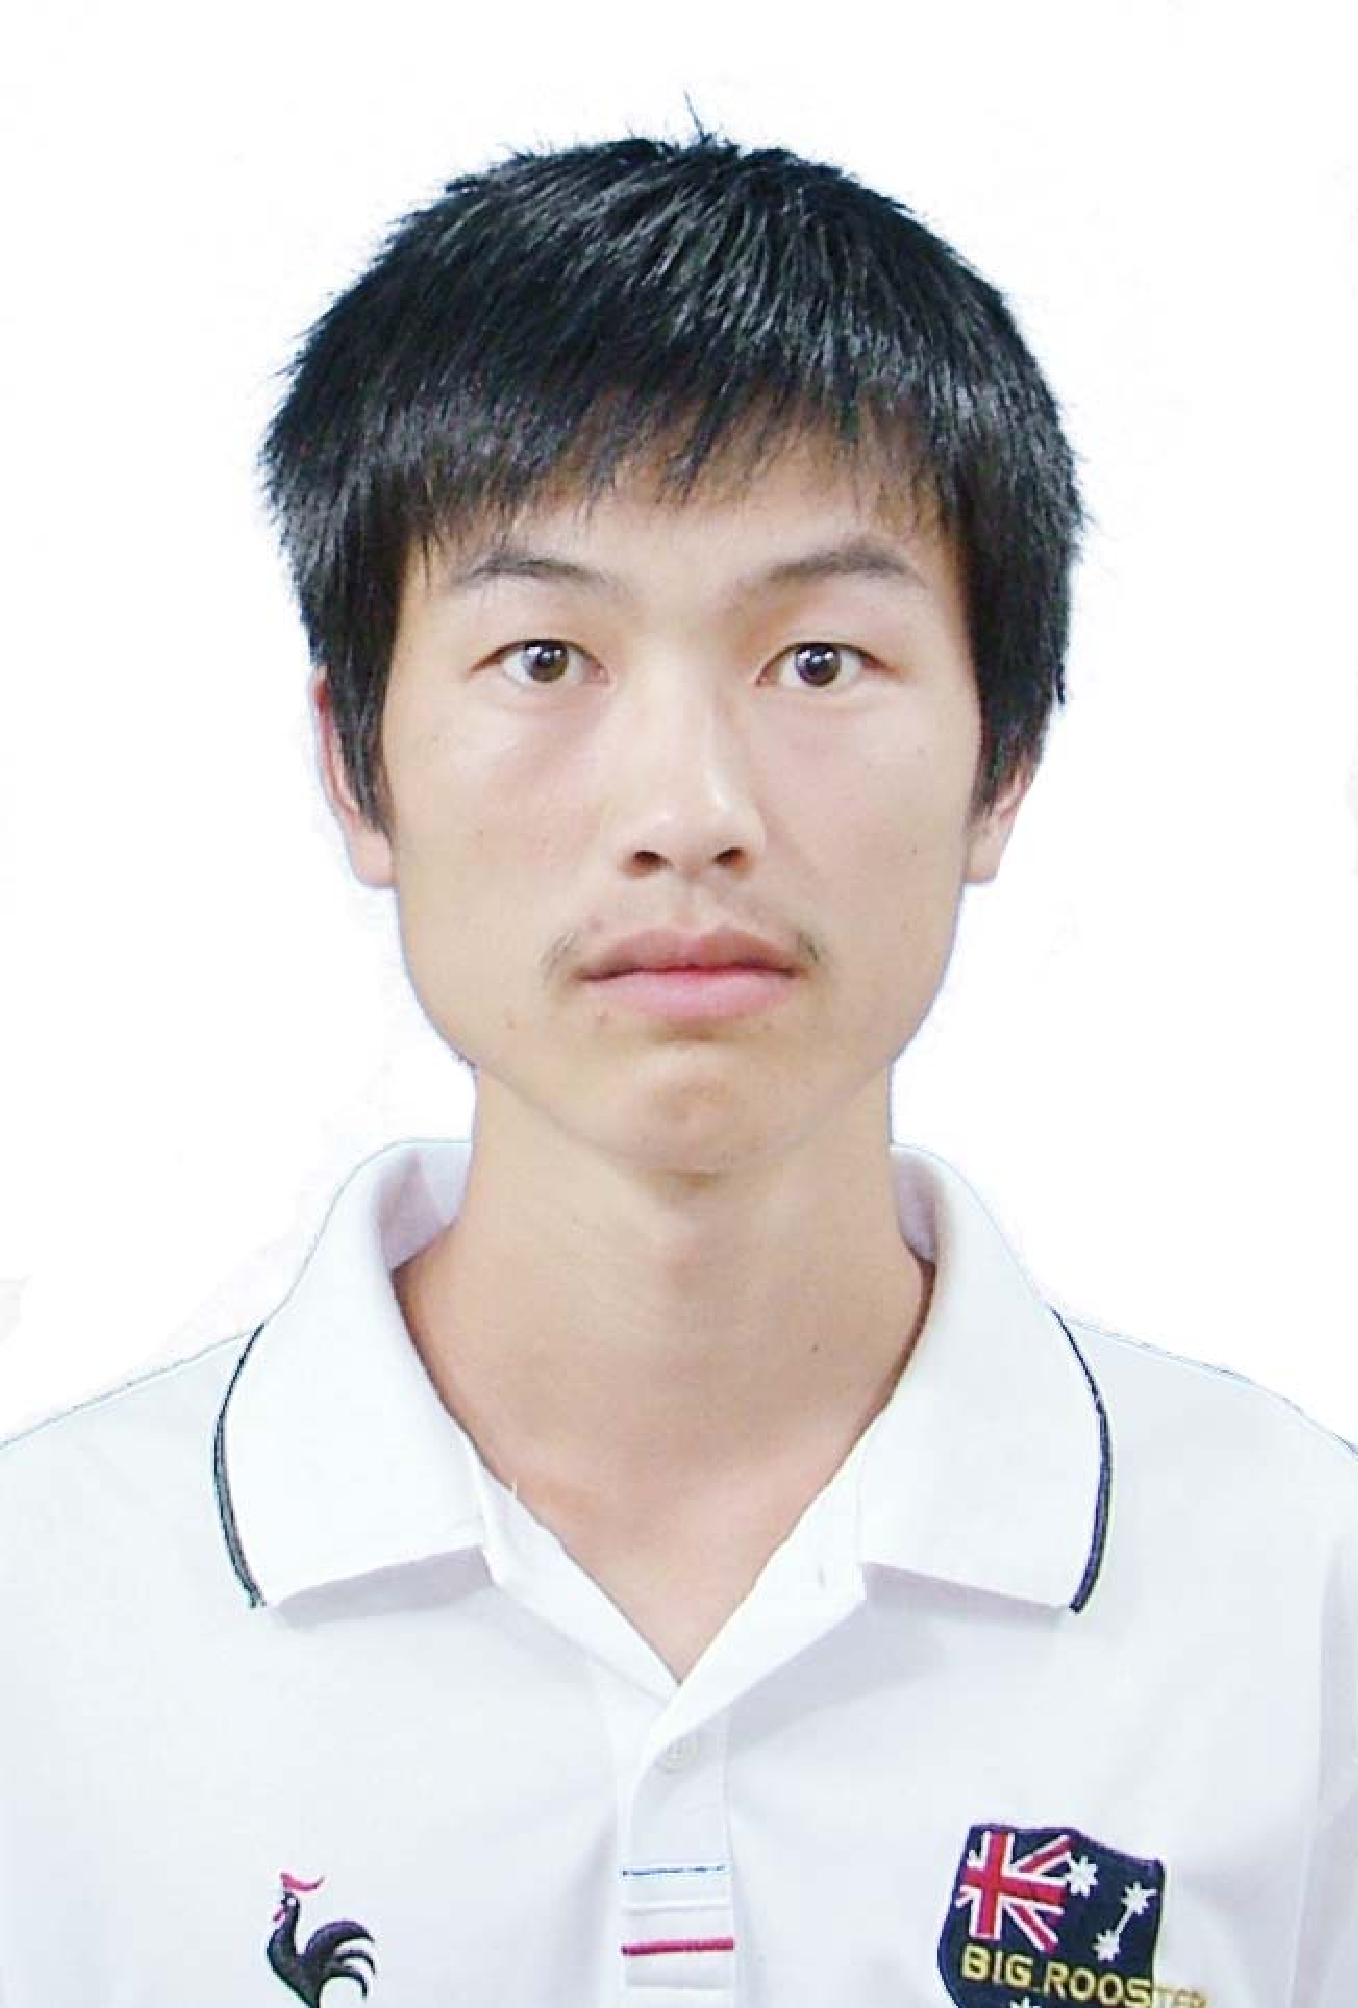
\includegraphics[width=1in,height=1.25in,clip,keepaspectratio]{photos/zhangjing.pdf}}]
	{Jing Zhang} is currently a graduate student at the College of Computer Science and Technology, Zhejiang University (ZJU). He received his B.Sc. from Huazhong University of Science and Technology (HUST) in 2017. His research interests include heterogeneous computing and data management.
\end{IEEEbiography}
\vspace*{-2\baselineskip}

\begin{IEEEbiography}[{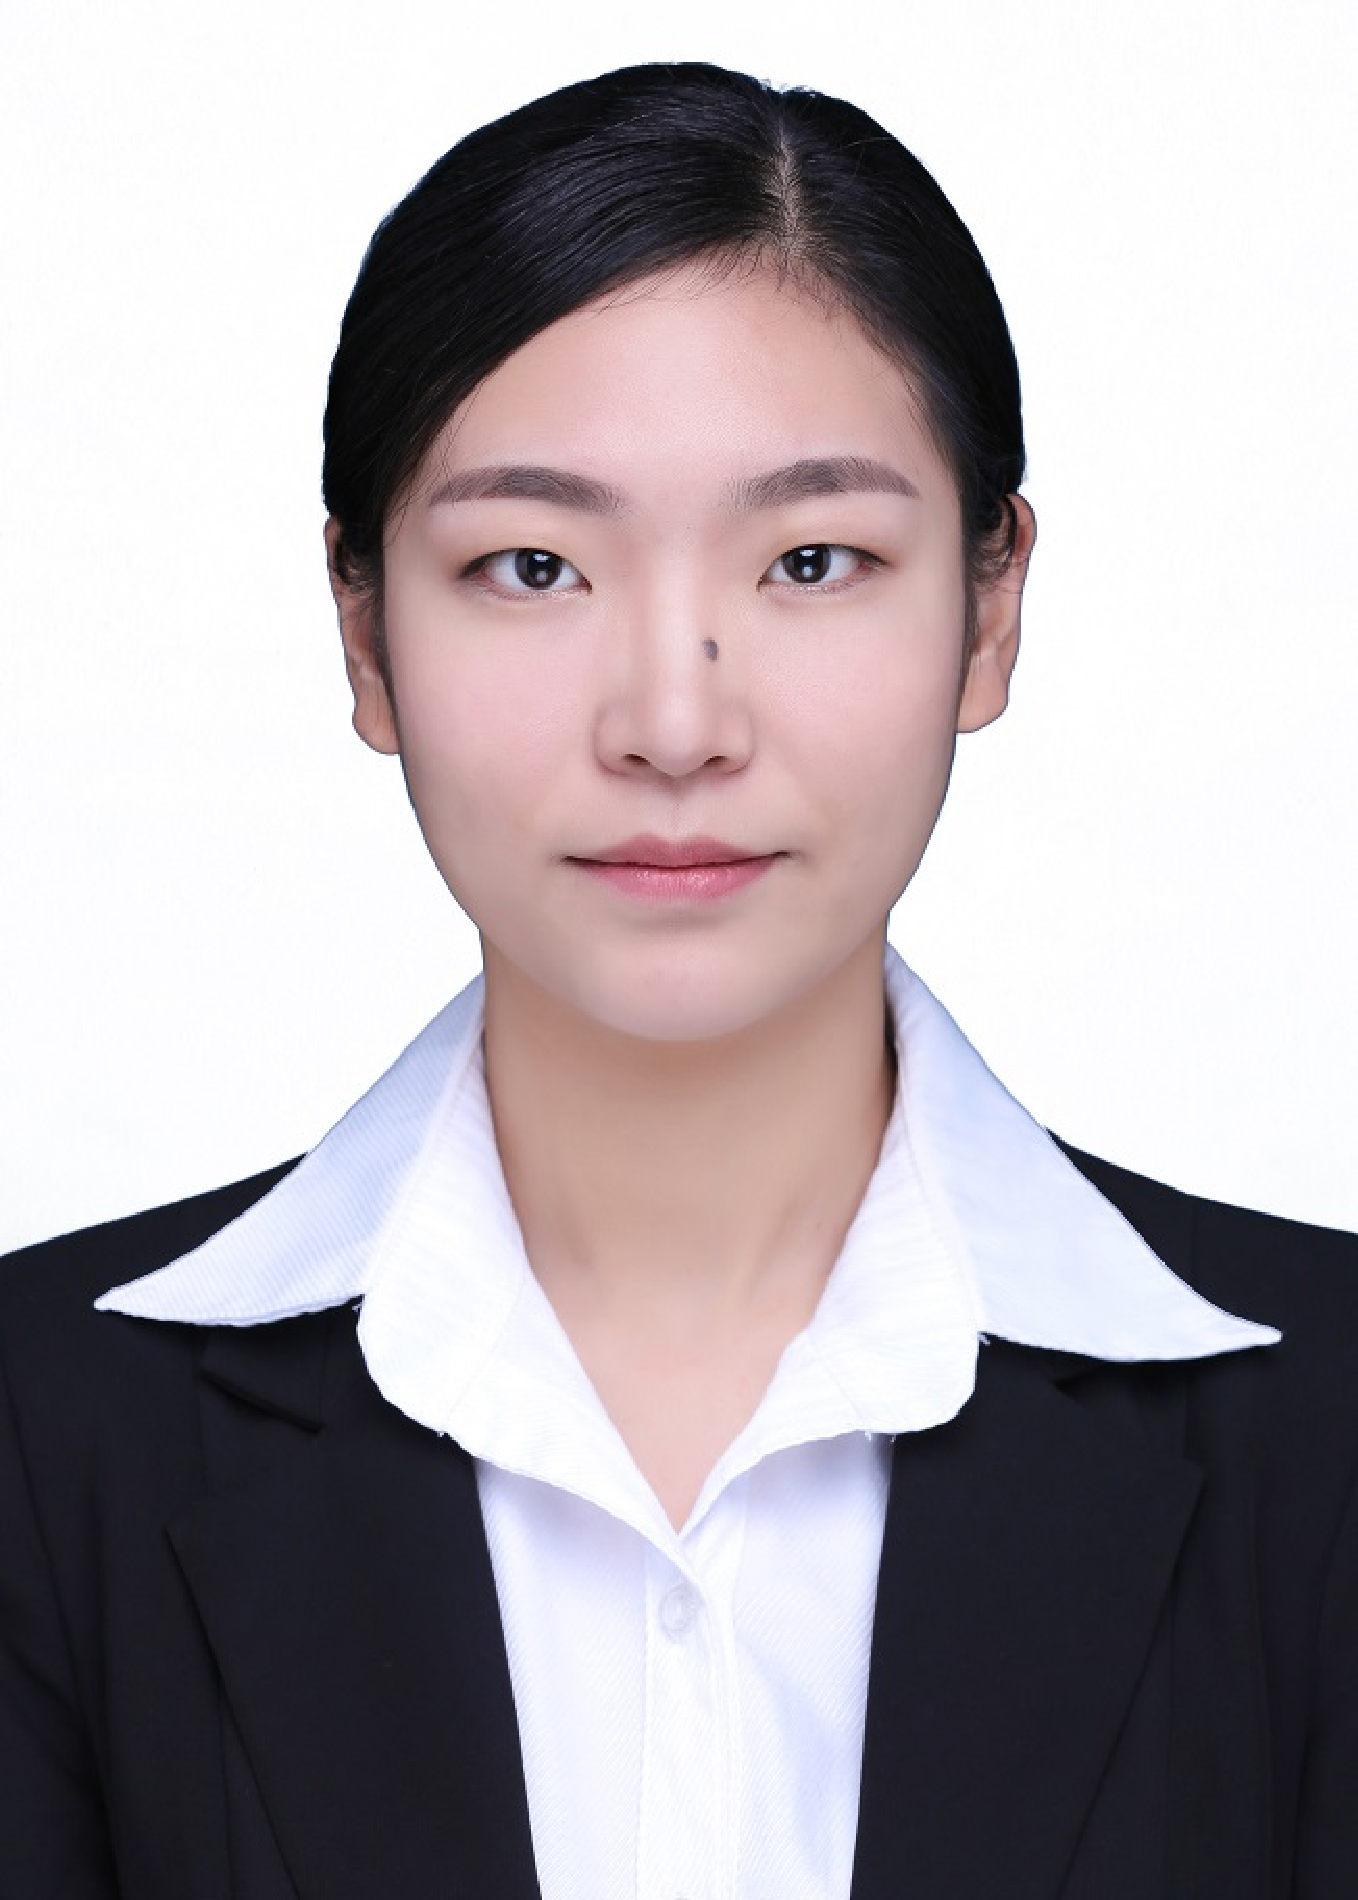
\includegraphics[width=1in,height=1.25in,clip,keepaspectratio]{photos/liuyue.pdf}}]
	{Yue Liu} is currently a graduate student at the College of Computer Science and Technology, Zhejiang University (ZJU). She received her B.Eng. in the Internet of Things from Hunan University (HNU) in 2017. Her research interests include heterogeneous computing and data management.
\end{IEEEbiography}
\vspace*{-2\baselineskip}

\begin{IEEEbiography}[{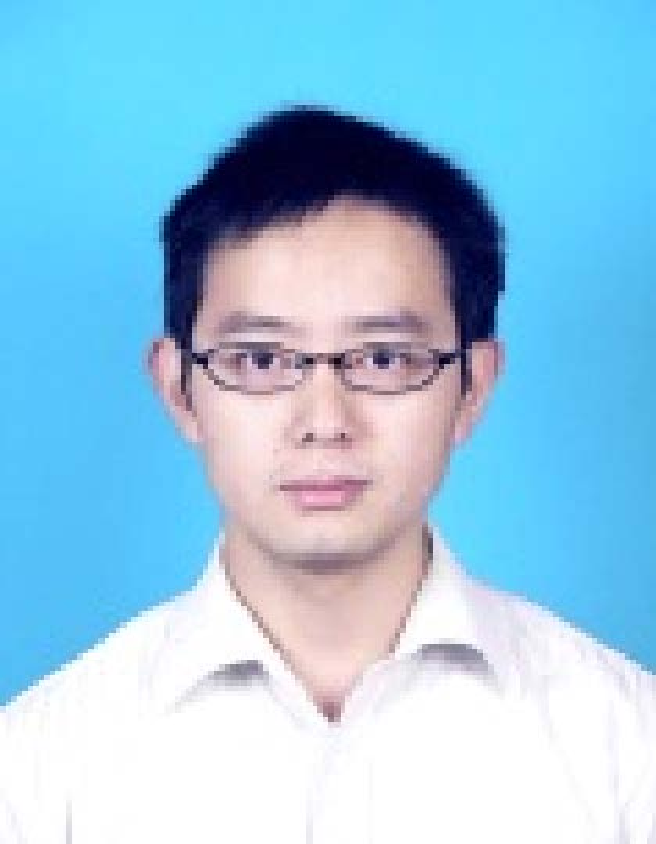
\includegraphics[width=1in,height=1.25in,clip,keepaspectratio]{photos/lvzheng.pdf}}]
	{Zheng Lyu} is now a staff engineer at Alibaba group, and responsible for development of GPU databases. He received his PhD in communication and information system from Shanghai institute of microsystem and information technology, Chinese Academy of Sciences in 2012. He mainly works in the area of high performance computing and his major research interest is heterogeneous computing in database system.
\end{IEEEbiography}
\vspace*{-2\baselineskip}

\begin{IEEEbiography}[{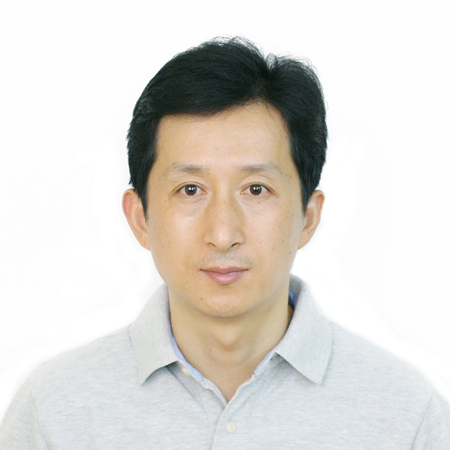
\includegraphics[width=1in,height=1.25in,clip,keepaspectratio]{photos/huang.pdf}}]
	{Zhongdong Huang} is an associate professor in the College of Computer Science and Technology, Zhejiang University. He received his B.Sc in Telecommunication and PhD degree in Computer Science from Zhejiang University in 1989 and 2003 respectively. His research interests include big data analytics and database systems.
\end{IEEEbiography}
\vspace*{-2\baselineskip}

\begin{IEEEbiography}[{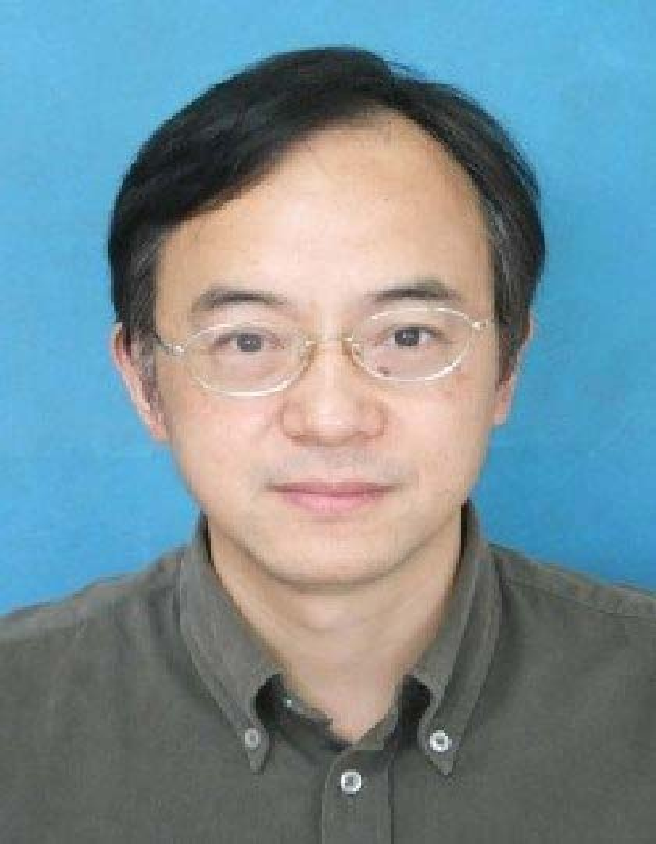
\includegraphics[width=1in,height=1.25in,clip,keepaspectratio]{photos/sun.pdf}}]
	{Jianling Sun} is a professor at the School of Computer Science and Technology. He received his PhD degree in computer science from Zhejiang University, China in 1993. His research interests include database systems, distributed computing, and machine Learning. He currently serves as the director of the Lab of Next Generation Database Technologies of Alibaba-Zhejiang University Joint Institute of Frontier Technologies. 
\end{IEEEbiography}
\vspace*{-2\baselineskip}

\end{document}
